\documentclass[journal]{IEEEtran}

% --- Preamble ---
% --- Essential Packages ---
\usepackage[utf8]{inputenc} % Input encoding
\usepackage[T1]{fontenc}    % Font encoding for better hyphenation
\usepackage{amsmath}
\usepackage{amssymb}        % Math symbols
\usepackage{amsfonts}       % Math fonts
\usepackage{amsthm}         % Theorem environments
\usepackage{bm}             % Bold math symbols (\bm)
\usepackage{graphicx}       % Include graphics
\usepackage{microtype}      % Improved typography and justification
\usepackage{cite}           % Handles citations like [1]-[3]
\usepackage{soul}           % For \hl{} highlighting
\usepackage{siunitx}        % For \sisetup and S column type
\usepackage{multirow}       % Multi-row cells in tables
\usepackage{booktabs}       % Nicer tables
\usepackage{textcomp}       % Additional text symbols
% --- Optional/Situational Packages ---
\usepackage{tabularx}
\usepackage[absolute,overlay]{textpos}
\usepackage{algorithm}
\usepackage{algpseudocode}
\usepackage{enumitem}
\usepackage[usenames,dvipsnames]{xcolor}
\usepackage{hyperref}

\newtheorem{theorem}{Theorem}
\newtheorem{definition}{Definition}
\newtheorem{lemma}{Lemma}

\sethlcolor{yellow}

\begin{document}

% === Section: 02_title.tex ===
% Title and author
\title{DyFlow-JEPA: Dynamical Flow Matching in Joint Embeddings for Anomaly Detection in Multi-Sensor IoT and Remote Sensing Telemetry}

\author{%
  \begin{tabular}{ccc}
    Andre Williams & Imadeldin Mahgoub & Hamid Akbarian\\
    \textit{Florida Atlantic University} & \textit{Florida Atlantic University} & \textit{Florida Atlantic University} \\
    \textit{Department of EECS} & \textit{Department of EECS} & \textit{Department of EECS} \\
    \textit{Boca Raton, US} & \textit{Boca Raton, US} & \textit{Boca Raton, US} \\
    \textit{andrewilliam2018@fau.edu} & \textit{mahgoubi@fau.edu} & \textit{hakbaria@fau.edu}
  \end{tabular}
}

% Running header guidance
\markboth{IEEE Transactions on Neural Networks and Learning Systems, SUBMISSION FOR REVIEW}%
{Submission}

\maketitle

% === Section: 03_abstract.tex ===
\begin{abstract}
Unsupervised anomaly detection in multi-sensor Internet-of-Things (IoT) networks and remote sensing telemetry supports operational health monitoring across aerospace systems, planetary exploration, cyber-physical infrastructure, and wearable sensing. However, detecting operational faults from sensor streams presents key challenges: reconstructive deep models (e.g., Autoencoders, Masked Transformers) often fit high-frequency sensor noise; heuristic contrastive detectors can distort state boundaries; and deterministic predictors collapse to the conditional mean across multi-branching dynamics. To address these limitations under edge computational budgets, we propose DyFlow-JEPA (Dynamical Flow-Matching Joint-Embedding Predictive Architecture), a continuous self-supervised framework for unsupervised anomaly detection in multi-sensor and remote sensing telemetry. DyFlow-JEPA frames anomaly detection as tangent velocity vector field modeling on a regularized latent dynamical manifold. DyFlow-JEPA pairs a causal context encoder with an Exponential Moving Average (EMA) target encoder, training a continuous velocity network via Optimal Transport Conditional Flow Matching (OT-CFM) regularized by non-contrastive variance and spectral covariance penalties to prevent representation collapse without synthetic negative sampling. For edge inference, we evaluate a single-pass Deterministic Midpoint Velocity Discrepancy at $t=0.5$, whitened by an empirical Mahalanobis precision tensor and thresholded via Extreme Value Theory (EVT / SPOT) under the Pickands-Balkema-de Haan theorem. Benchmarking across 1,300 model-channel runs on 11 real-world telemetry datasets comprising 130 continuous channels demonstrates that DyFlow-JEPA outperforms deep baselines (TimesNet, TranAD, Anomaly Transformer, DCdetector, NCAD), achieving a channel-weighted Point-F1 of $0.2389$ (+52.5\% over TimesNet and +56.2\% over TranAD) and an unweighted dataset macro Point-F1 of $0.1921$. Phase-space dynamical analyses confirm that DyFlow-JEPA models nominal multi-sensor physical dynamics as stable limit cycles, providing interpretable state trajectories and suppressing false alarms.
\end{abstract}


\begin{IEEEkeywords}
Multi-Sensor IoT, Remote Sensing Telemetry, Spacecraft Telemetry, Anomaly Detection, Joint-Embedding Predictive Architecture (JEPA), Flow Matching, Optimal Transport, Continuous Dynamical Systems, Wearable Edge Sensing, Extreme Value Theory.
\end{IEEEkeywords}

% === Section: 04_intro.tex ===
\section{Introduction}
\label{sec:intro}

Autonomous anomaly detection in multi-sensor telemetry monitors operational health across aerospace systems, Earth observation, cyber-physical infrastructure, and wearable digital healthcare \cite{meng2019spacecraft, chalapathy2019deep}. In remote sensing deployments (such as the NASA Soil Moisture Active Passive (SMAP) satellite, Mars Science Laboratory (MSL) rovers, industrial IoT facilities, and wearable biometric sensor arrays), dozens to hundreds of continuous telemetry channels concurrently track electrical power buses, thermal gradients, mechanical vibrations, and kinematics \cite{Hundman2018b}. When sensor faults or operational breakdowns emerge at the edge, monitoring systems must identify dynamical anomalies before hardware damage occurs \cite{cuellar2024explainable}.

\subsection{Challenges in Modeling Multi-Sensor Telemetry}
From a physical perspective, multi-sensor telemetry reflects the state trajectory of an underlying continuous physical system $\dot{x}(t) = \mathbf{f}(x(t))$. However, attempting to model dynamical equations directly in raw observation space presents four main challenges on edge devices:
\begin{enumerate}[leftmargin=*]
    \item \textit{Numerical Instability in Empirical Differentiation:} Estimating instantaneous time derivatives $\dot{x} \approx \frac{\Delta x}{\Delta t}$ directly on discrete, noise-corrupted sensor streams amplifies high-frequency measurement noise, destabilizing numerical trajectory tracking.
    \item \textit{Partial Observability \& Unmeasured Internal States:} Remote sensing telemetry captures only a noisy surface projection of unmeasured thermodynamic, electrical, and environmental states, violating full-state observability.
    \item \textit{High-Dimensional Cross-Sensor Coupling:} In multi-sensor IoT pods ($K \ge 50$), complex cross-channel dependencies and non-linear interactions cannot be adequately represented by rigid functional forms in raw signal space.
    \item \textit{Non-Stationary Downlink \& Operational Drift:} Edge IoT and satellite systems undergo discrete operational mode transitions (e.g., orbital day/night thermal cycling, thruster firings, Parkinsonian gait freezing, cloud server garbage collection) that cause continuous distribution drift.
\end{enumerate}

\subsection{Limitations of Deep Anomaly Detectors}
To bypass explicit equation modeling, deep learning architectures have emerged as data-driven alternatives, yet they remain constrained by three primary limitations:
\begin{enumerate}[leftmargin=*]
    \item \textit{Signal-Level Noise Memorization:} Traditional generative models (e.g., Autoencoders, VAEs, Masked Transformers) minimize point-level $L_1/L_2$ errors in raw signal space \cite{Hundman2018b, xu2022anomaly, wu2023timesnet}. Because reconstruction loss penalizes every point discrepancy equally, autoencoders expend substantial capacity memorizing high-frequency stochastic sensor jitter rather than learning the macro-scale dynamical laws governing nominal transitions.
    \item \textit{Limitations of Synthetic Contrastive Perturbations:} Contrastive frameworks like Neural Contextual Anomaly Detection (NCAD) \cite{carmona2021neural} train encoders via Contextual Outlier Exposure (COE) using heuristic synthetic perturbations (e.g., Gaussian noise spikes, sequence splicing). However, real physical faults manifest as subtle shifts away from nominal operating dynamics. Synthetic injections distort the learned embedding geometry, inducing artificial decision boundaries that produce false alarms on continuous physical streams.
    \item \textit{Conditional Mean Collapse in Multi-Branch Dynamics:} Deterministic predictive encoders trained with MSE loss $\mathbb{E}[\|\hat{z} - z\|^2]$ are mathematically constrained to predict the \textit{conditional mean} $\mathbb{E}[z_{\text{tgt}} \mid z_{\text{ctx}}]$. When physical systems possess multiple valid operational branches, the conditional mean lands in low-probability regions of representation space, triggering false alarms during legitimate multi-modal state transitions.
\end{enumerate}

\subsection{Our Approach: Dynamical Flow Matching for Edge Telemetry}
To address raw-space numerical noise and the reconstruction/collapse trade-offs of deep baselines, we evaluate a deterministic predictive baseline (Point-JEPA) and propose DyFlow-JEPA (Dynamical Flow-Matching Joint-Embedding Predictive Architecture). While flow matching has been explored in generative vision and robotics, we formulate flow matching for unsupervised anomaly detection in multi-sensor telemetry. Rather than integrating stiff trajectories in raw sensor space or reconstructing noisy waveforms, DyFlow-JEPA embeds the multi-sensor system into an abstract representation space and learns the continuous tangent velocity vector field of the nominal physical attractor manifold via Optimal Transport Conditional Flow Matching (OT-CFM) \cite{lipman2022flow}.

\begin{figure*}[t]
    \centering
    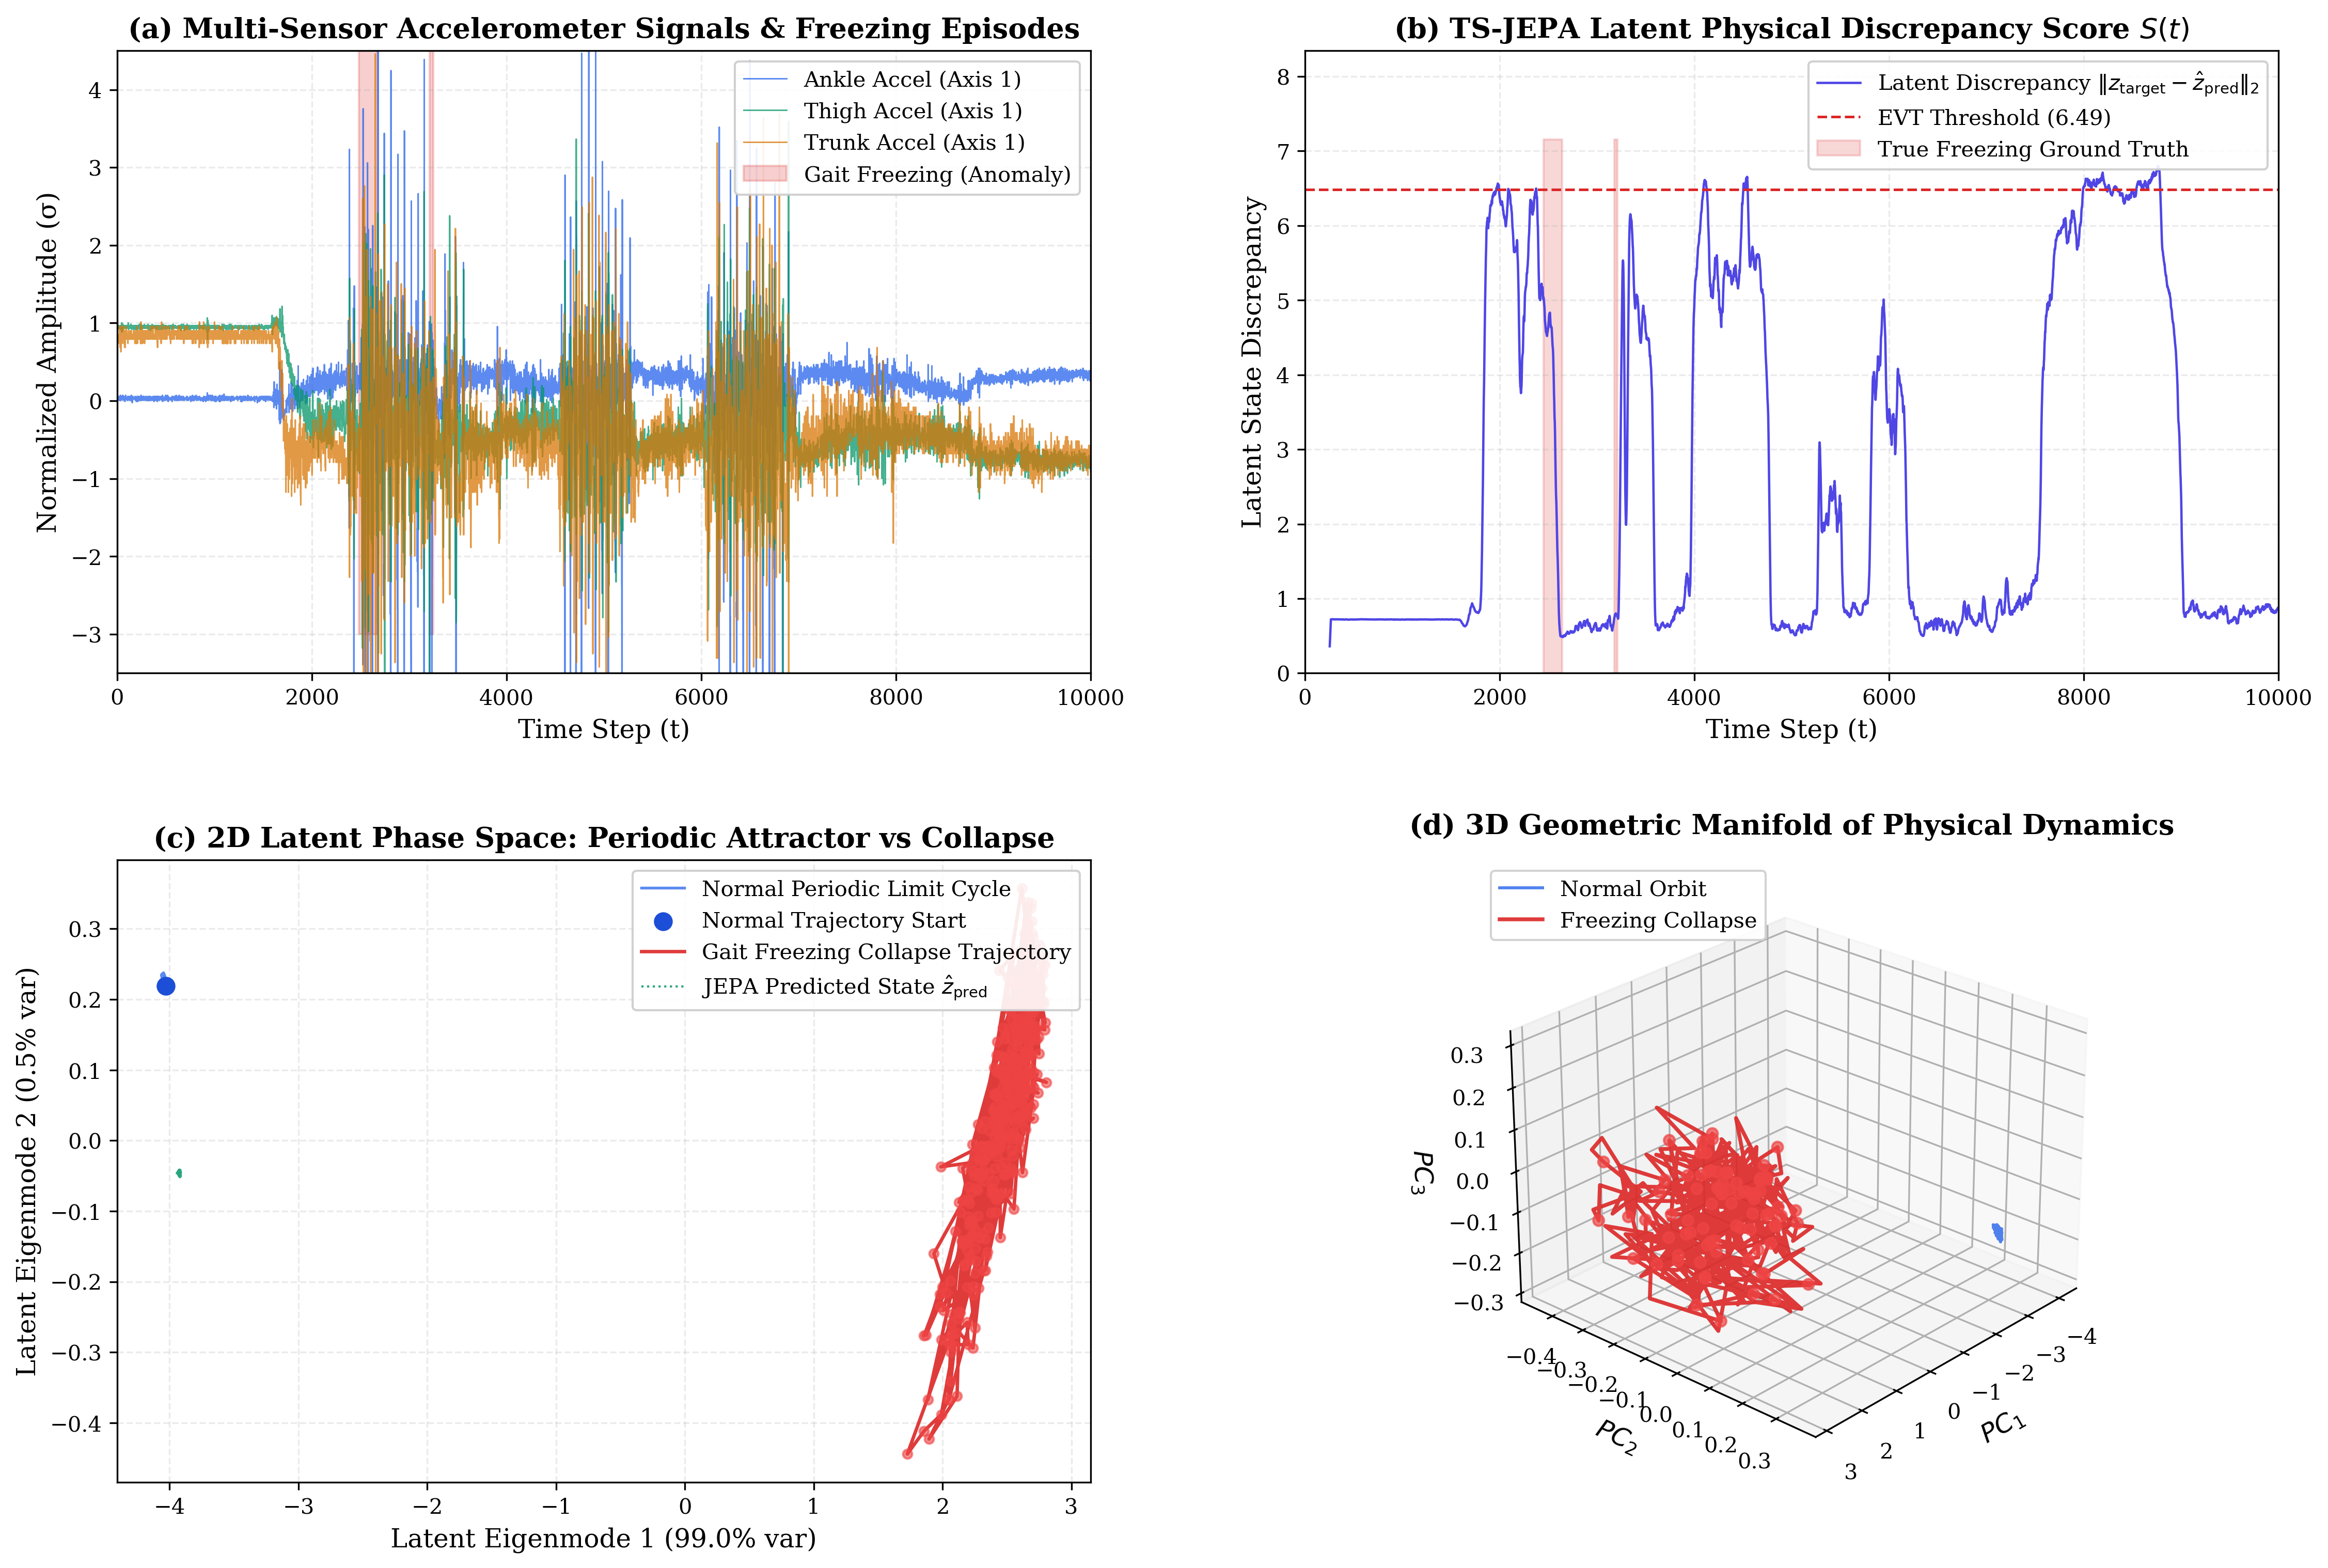
\includegraphics[width=0.95\linewidth]{figures/daphnet_phase_space_attractor.png}
    \caption{Phase-space dynamical analysis and anomaly detection with baseline Point-JEPA. (a) Raw multi-sensor accelerometry with ground-truth freezing-of-gait anomalies. (b) Point-JEPA latent discrepancy score $S(t) = \|z_{\text{tgt}} - \hat{z}_{\text{pred}}\|_2$ with EVT-calibrated decision threshold. (c) 2D and (d) 3D latent phase space: nominal dynamics form a stable periodic limit cycle (blue orbit), which the predictive encoder anticipates with near-zero error (green dashed line). When an anomaly occurs, the trajectory rapidly diverges from the attractor manifold (red line), generating a sharp, unambiguous anomaly signal.\label{fig:phase_space_attractor}}
\end{figure*}


As illustrated in Figure~\ref{fig:phase_space_attractor}, Point-JEPA maps nominal system behavior into stable limit-cycle attractors in representation space. In DyFlow-JEPA, a causal dilated Temporal Convolutional Network (TCN) or Patch Transformer context encoder processes historical context $x_{\text{ctx}}$, while a continuous flow velocity network $v_\psi(z_t, t, z_{\text{ctx}})$ models the probability paths leading to target representations $z_{\text{tgt}}$. The representation space is regularized via non-contrastive VICReg (Invariance, Variance hinge, Covariance decorrelation) \cite{bardes2021vicreg} to prevent dimensional collapse.

During inference on edge hardware, anomalous telemetry is detected by measuring the Deterministic Midpoint Velocity Discrepancy at $t=0.5$, whitened by an empirical Mahalanobis precision tensor $\mathbf{\Sigma}^{-1}$. Finally, Extreme Value Theory (EVT / SPOT) tail calibration \cite{siffer2017anomaly} establishes a decision threshold under the Pickands-Balkema-de Haan theorem, eliminating heuristic threshold tuning.

\subsection{Key Contributions}
The primary contributions of this work are as follows:
\begin{itemize}[leftmargin=*]
    \item \textit{Continuous Dynamical Flow Matching for Multi-Sensor Telemetry:} We formulate a continuous flow-matching joint-embedding framework for unsupervised anomaly detection in multi-sensor telemetry, modeling fault detection as continuous tangent velocity field learning on latent dynamical manifolds and avoiding conditional-mean collapse on multi-branching physical systems.
    \item \textit{Physical Attractor Geometry \& Non-Contrastive Regularization:} We formulate Optimal Transport Conditional Flow Matching within an EMA-regularized latent space, constrained by variance hinge and spectral covariance penalties to preserve dimensional rank across coupled sensor arrays without synthetic outlier injection.
    \item \textit{Deterministic Midpoint Evaluation \& Statistical Calibration:} We derive a zero-variance, single-pass deterministic midpoint velocity discrepancy metric ($t=0.5$) with second-order Taylor error bounds, coupled with Mahalanobis covariance whitening and Generalized Pareto Distribution (EVT / SPOT) extreme value calibration to set threshold-free decision alarms under low edge inference latency ($3.47$s).
    \item \textit{Multi-Sensor Telemetry Benchmark Evaluation:} Evaluated across 11 telemetry benchmark datasets comprising 130 continuous channels spanning four domain families (satellite remote sensing, wearable IoT, industrial testbeds, and smart infrastructure), DyFlow-JEPA outperforms deep baselines (TimesNet, TranAD, Anomaly Transformer, DCdetector, NCAD) under both channel-weighted and unweighted dataset macro metrics.
\end{itemize}



The remainder of this paper is structured as follows. Section~\ref{sec:related} reviews related work across equation discovery, reconstruction, contrastive learning, and JEPAs. Section~\ref{sec:dataset} describes the multi-sensor IoT and remote sensing benchmark suite. Section~\ref{sec:proposed_method} details the DyFlow-JEPA architecture, Optimal Transport flow matching, manifold regularization, and Mahalanobis EVT scoring. Section~\ref{sec:exp} presents the experimental setup, baselines, and grand benchmark evaluation. Section~\ref{sec:ablations} provides systematic ablation studies on loss formulations, latent capacity, and velocity discrepancy. Section~\ref{sec:results} discusses domain-by-domain insights, point-adjustment dynamics, and phase-space attractors. Finally, Section~\ref{sec:conclusion} concludes the paper and outlines future directions.

% === Section: 05_related.tex ===
\section{Related Work}
\label{sec:related}

Unsupervised time-series anomaly detection spans dynamical equation discovery, reconstructive generative modeling, contrastive representation learning, and predictive world models. This section reviews these approaches and positions DyFlow-JEPA.

\subsection{Continuous Dynamical Systems and Flow Matching}
The physical modeling of multi-sensor telemetry has long sought to capture system behavior as continuous dynamical trajectories governed by differential equations $\dot{x}(t) = \mathbf{f}(x(t))$ \cite{brunton2016discovering}.
\begin{itemize}[leftmargin=*]
    \item \textit{Neural Ordinary Differential Equations (Neural ODEs) \cite{chen2018neural}:} Parameterize continuous velocity fields using neural networks $\frac{dx}{dt} = f_\theta(x(t), t)$ and solve trajectories via numerical ODE integrators. While Neural ODEs learn flexible vector fields, fitting them directly in raw sensor space forces numerical solvers to integrate through high-frequency stochastic sensor noise, leading to numerical stiffness, slow training, and extreme sensitivity to measurement noise.
    \item \textit{Conditional Flow Matching (CFM) \cite{lipman2022flow, tong2023improving}:} Continuous Normalizing Flows and Optimal Transport Conditional Flow Matching (OT-CFM) train neural velocity vector fields $v_\psi(z_t, t)$ along straight probability paths. Stochastic interpolant frameworks \cite{albergo2022building} provide efficient simulation-free training objectives. DyFlow-JEPA couples Optimal Transport Flow Matching with non-contrastive Joint-Embedding representations, learning continuous dynamical vector fields purely in regularized latent space without raw-space noise integration.
\end{itemize}

\subsection{Reconstruction-Based Detection}
The predominant deep learning approach in time-series anomaly detection relies on learning nominal patterns through raw signal reconstruction. Hundman et al. \cite{Hundman2018b} introduced LSTM-based prediction coupled with non-parametric dynamic thresholding for NASA spacecraft telemetry (SMAP/MSL). Modern architectures incorporate specialized attention and frequency-domain transformations:
\begin{itemize}[leftmargin=*]
    \item \textit{Anomaly Transformer \cite{xu2022anomaly}:} Introduces Anomaly-Attention to quantify the \textit{Association Discrepancy} between local prior Gaussian kernel associations and global series self-attention. While effective for isolated point anomalies, it couples discrepancy with point-level waveform reconstruction.
    \item \textit{TimesNet \cite{wu2023timesnet}:} Decomposes 1D multivariate time series into 2D temporal variations using Fast Fourier Transform (FFT) periodicity discovery and 2D Inception blocks. However, optimizing point-level 2D reconstruction makes it susceptible to over-fitting high-frequency sensor noise.
    \item \textit{TranAD \cite{tuli2022tranad}:} Employs a two-phase adversarial Transformer with sub-series attention and focus scoring to amplify subtle reconstruction errors, but remains vulnerable to phase-drift in continuous dynamical systems.
\end{itemize}

Reconstructive methods share a common vulnerability: \textit{signal-level reconstruction memorization}. Because loss functions optimize point-level $L_1$ or $L_2$ differences in raw signal space, reconstructive networks are biased toward fitting high-frequency stochastic noise rather than learning invariant dynamical laws. Furthermore, during sustained anomalies, corrupted observations contaminate the context window, causing the reconstructor to adapt and reconstruct the anomaly as the "new normal."

\subsection{Contrastive Learning and Representation-Based Detection}
To avoid reconstructing raw noise, contrastive methods learn discriminative representations by separating nominal sequences from anomalous perturbations:
\begin{itemize}[leftmargin=*]
    \item \textit{Neural Contextual Anomaly Detection (NCAD) \cite{carmona2021neural}:} Uses Temporal Convolutional Networks (TCNs) trained with Contextual Outlier Exposure (COE). Artificial synthetic anomalies (Gaussian noise, point spikes, trend shifts) are injected into training windows to create negative pairs. However, synthetic injections distort the physical dynamical manifold and fail to generalize to subtle real-world physical faults (e.g., gradual thermal dissipation or gait freezing).
    \item \textit{DCdetector \cite{yang2023dcdetector}:} Replaces reconstruction with multi-scale dual-attention (patch-wise and channel-wise) contrastive representation learning, maximizing cross-scale representation consistency. While DCdetector eliminates artificial injection heuristics, contrastive objectives require careful scale selection and representation pooling.
\end{itemize}

\subsection{Non-Contrastive Learning and Time-Series JEPAs}
Joint-Embedding Predictive Architectures (JEPA), originally proposed by LeCun \cite{lecun2022path} and demonstrated in computer vision by I-JEPA \cite{assran2023self} and V-JEPA \cite{bardes2024vjepa}, predict target representations from context in latent space. Non-contrastive regularizers like Barlow Twins \cite{zbontar2021barlow}, W-MSE \cite{ermolov2021whitening}, and VICReg \cite{bardes2021vicreg} prevent representation collapse without negative mining.

Recent works have extended joint-embedding predictive principles to time-series sequences:
\begin{itemize}[leftmargin=*]
    \item \textit{Time-Series JEPAs:} SC-JEPA / MTS-JEPA \cite{he2026scjepa} stabilizes latent predictive learning for time-series anomaly prediction using a multi-scale soft-codebook dictionary. T-SAR-JEPA \cite{woldesenbet2026tsarjepa} applies self-supervised latent prediction to Synthetic Aperture Radar (SAR) amplitude time series. CF-JEPA \cite{lee2026cfjepa} employs mask-free forward prediction with asymmetric encoders for time-series representation learning. In cyber-physical and automotive domains, Girgis et al. \cite{girgis2026timeseries} explore time-series JEPAs for predictive remote control over capacity-constrained IoT channels, while Fertig et al. \cite{fertig2026online} investigate JEPA embeddings for online automotive sensor monitoring.
\end{itemize}
However, these time-series JEPA adaptations rely on deterministic point regression or discrete codebook quantization, which collapse to the conditional mean on stochastic, multi-branching physical systems.

\subsection{Flow Matching in Joint Embeddings (Vision, Control, and World Models)}
Recently, the integration of continuous flow matching into joint-embedding architectures has been applied to generative vision and reinforcement learning:
\begin{itemize}[leftmargin=*]
    \item \textit{Generative Vision and Multimodal Synthesis:} D-JEPA \cite{xie2024djepa} pioneered the use of flow matching and diffusion objectives within JEPA predictors to replace discrete next-token prediction for continuous image, video, and audio generation. Concurrently, JEPA-T \cite{wang2025jepat} integrated flow-matching feature predictors with cross-attention for text-to-image synthesis.
    \item \textit{World Models and Robotic Control:} In reinforcement learning, Qantara \cite{qantara2026} introduced Bridge-Flow training for multi-task JEPA control, while concurrent work by Madaan et al. \cite{flowjepa2026world} investigated flow matching for trajectory-level state rollouts in latent dynamics world models.
\end{itemize}

Prior work applies flow matching to generative image synthesis and action-conditioned robotic state transitions. In contrast, DyFlow-JEPA applies continuous flow matching within joint embeddings to unsupervised multivariate time-series anomaly detection. Rather than optimizing action-conditioned rollouts or pixel generation, DyFlow-JEPA models the continuous tangent velocity field of physical dynamical attractors in multi-sensor telemetry, evaluating it with a deterministic midpoint discrepancy estimator, Mahalanobis mode whitening, and Extreme Value Theory (EVT / SPOT) tail calibration.

\subsection{Positioning and Method Design}
DyFlow-JEPA combines continuous dynamical modeling and joint-embedding self-supervised learning through four key components:
\begin{enumerate}[leftmargin=*]
    \item \textit{Continuous Latent Vector Field Modeling:} Instead of raw-space differential equation solving or deterministic point regression, DyFlow-JEPA learns the continuous tangent velocity field of the physical manifold via Optimal Transport Conditional Flow Matching directly in regularized latent space.
    \item \textit{Non-Contrastive Manifold Regularization:} Replaces synthetic negative injection heuristics with non-contrastive variance and spectral covariance penalties, precluding dimensional collapse while preserving smooth attractor geometry.
    \item \textit{Deterministic Midpoint Velocity Discrepancy:} Evaluates the velocity field at the Optimal Transport midpoint ($t=0.5$), providing an efficient, zero-Monte-Carlo-variance proxy for trajectory deviation whitened by an empirical Mahalanobis precision tensor.
    \item \textit{Extreme Value Tail Calibration:} Applies Extreme Value Theory (EVT / SPOT) \cite{siffer2017anomaly} under the Pickands-Balkema-de Haan theorem \cite{balkema1974residual} to fit Generalized Pareto tails on nominal velocity residuals, setting decision boundaries without manual threshold tuning.
\end{enumerate}

% === Section: 06_dataset.tex ===
\section{Multi-Sensor IoT and Remote Sensing Benchmark Suite}
\label{sec:dataset}

To evaluate DyFlow-JEPA across diverse edge, cyber-physical, and orbital sensing dynamics, our benchmark suite comprises 11 datasets spanning 130 continuous telemetry channels sourced from NASA spacecraft archives \cite{Hundman2018b}, the PhysioNet biomedical database \cite{bachlin2010wearable}, TimeEval \cite{schmidl2022anomaly}, and mTSBench \cite{zhou2026mtsbench}. We group these channels into four IoT and remote sensing domains:

\subsection{Domain 1: Satellite and Planetary Remote Sensing (78 Channels)}
\begin{enumerate}[leftmargin=*]
    \item \textit{NASA SMAP Earth Observation Satellite \cite{Hundman2018b} (51 channels):} Continuous power, thermal, and attitude telemetry from the Soil Moisture Active Passive (SMAP) spacecraft tracking solar array currents, bus voltages, battery temperatures, and thruster status subject to radiation upsets and operational mode shifts.
    \item \textit{NASA MSL Curiosity Rover \cite{Hundman2018b} (26 channels):} Environmental and robotic actuator telemetry from the Mars Science Laboratory (MSL) rover monitoring drive motor currents, joint angles, arm kinematics, and power subsystem faults during planetary exploration.
    \item \textit{SWAN Coastal Hydro-Acoustic Remote Sensing (1 channel):} Surface water and marine acoustic telemetry tracking sudden ocean surges and wave anomalies.
\end{enumerate}

\subsection{Domain 2: Wearable IoT and Edge Biometrics (26 Channels)}
\begin{enumerate}[leftmargin=*]
    \item \textit{Daphnet Wearable Body Sensor Network \cite{bachlin2010wearable} (26 channels):} High-frequency tri-axial accelerometry from wearable body sensor nodes (placed on the shank, thigh, and trunk; 9 continuous dimensions per subject) tracking Freezing-of-Gait (FoG) breakdown events in Parkinson's patients.
\end{enumerate}

\subsection{Domain 3: Industrial IoT and Cyber-Physical Testbeds (16 Channels)}
\begin{enumerate}[leftmargin=*]
    \item \textit{GHL Industrial Separation Plant (14 channels):} Multi-phase gas-oil-water separation industrial process telemetry monitoring tank levels, flow rates, and valve control faults.
    \item \textit{Genesis Automation Testbed (1 channel):} Industrial manufacturing testbed telemetry tracking automated handling machinery faults.
    \item \textit{GECCO Water Distribution IoT (1 channel):} Physical water distribution process telemetry monitoring chemical and hydrological sensor measurements.
\end{enumerate}

\subsection{Domain 4: Smart Infrastructure and Environmental IoT (10 Channels)}
\begin{enumerate}[leftmargin=*]
    \item \textit{Room-Occupancy Environmental IoT \cite{candanedo2016accurate} (2 channels):} Multi-sensor ambient environmental IoT sensing ($\text{CO}_2$, light, temperature, humidity) tracking room-occupancy state switches.
    \item \textit{CICIDS Edge Network Telemetry (6 channels):} High-throughput network flow telemetry capturing edge gateway protocol dynamics and security anomalies (DDoS bursts and port scans).
    \item \textit{CalIt2 Campus Smart Traffic (1 channel):} Vehicle flow counts and speed telemetry at smart campus entry points during special events.
    \item \textit{Metro Interstate Highway Traffic (1 channel):} Traffic volume and environmental condition telemetry on smart highway corridors.
\end{enumerate}

In addition to the 130 primary benchmark channels, we evaluate the \textit{Exathlon Distributed Cloud Benchmark \cite{jacob2021exathlon} (30 channels)} in our ablation suite (Section~\ref{sec:ablations}). Exathlon captures high-dimensional execution traces from distributed Apache Spark clusters (JVM heap utilization, garbage collection pauses, memory leaks, and CPU thrashing), providing a testbed to evaluate target encoder momentum stability under non-stationary streaming drift.

Each benchmark channel provides pre-split training sequences (consisting exclusively of nominal operational behavior) and testing sequences containing labeled ground-truth anomalies. Continuous numeric features are standardized via training statistics ($\bm{\mu}_{\text{train}}, \bm{\sigma}_{\text{train}}$), flooring standard deviations at $\max(\bm{\sigma}, 10^{-2})$ to prevent division by zero during flat-line operational phases.

% === Section: 07_method.tex ===
\section{Method: DyFlow-JEPA}
\label{sec:proposed_method}

\begin{figure*}[t]
\centering
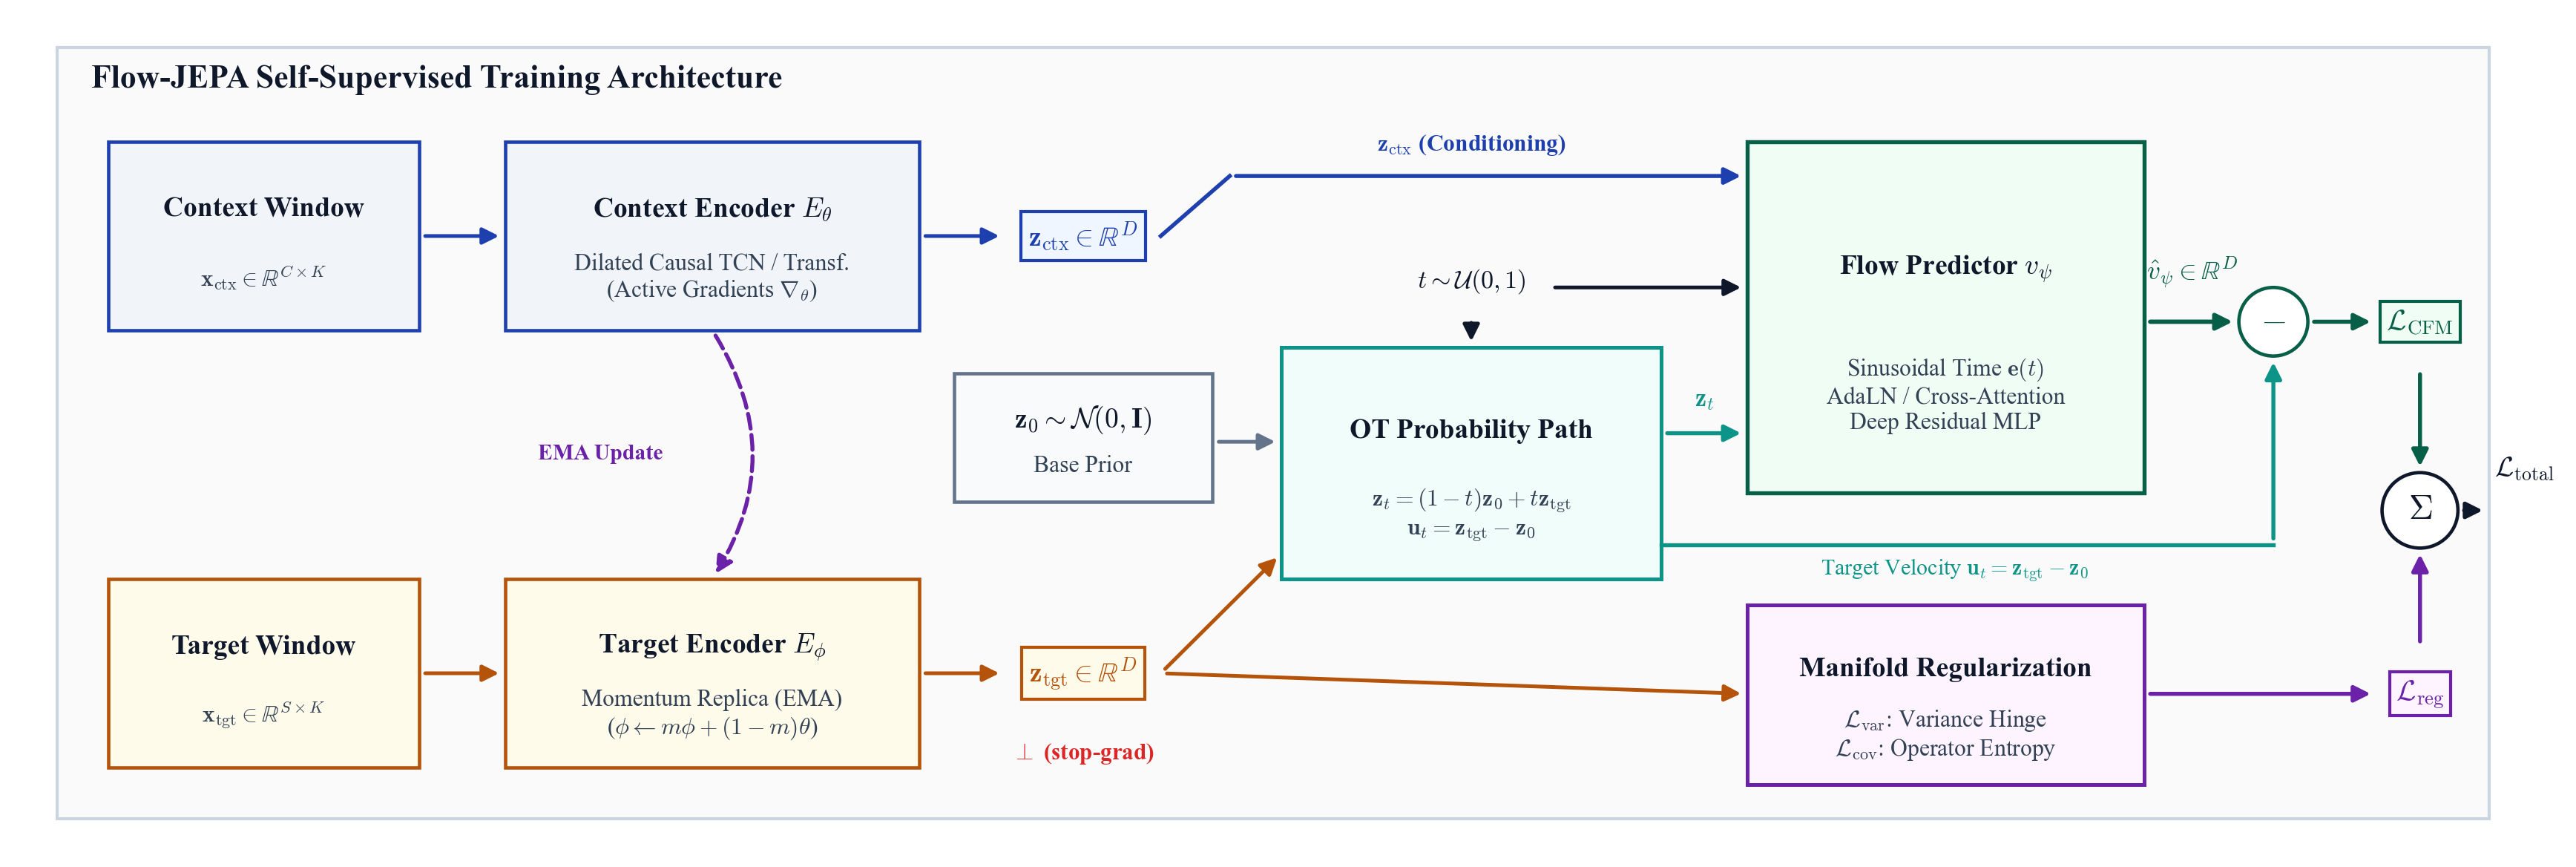
\includegraphics[width=\textwidth]{figures/flow_jepa_training.png}
\caption{DyFlow-JEPA self-supervised training architecture. The context window $\mathbf{x}_{\text{ctx}} \in \mathbb{R}^{C \times K}$ and target window $\mathbf{x}_{\text{tgt}} \in \mathbb{R}^{S \times K}$ are mapped to latent space by context encoder $E_\theta$ (trained with active gradients $\nabla_\theta$) and momentum target encoder $E_\phi$ (EMA replica with stop-gradient $\bot$). Straight Optimal Transport probability paths $\mathbf{z}_t = (1-t)\mathbf{z}_0 + t\mathbf{z}_{\text{tgt}}$ are sampled between base prior $\mathbf{z}_0 \sim \mathcal{N}(\mathbf{0}, \mathbf{I}_D)$ and target $\mathbf{z}_{\text{tgt}}$. The continuous flow predictor $v_\psi$ learns the instantaneous velocity field conditioned on $\mathbf{z}_{\text{ctx}}$ and sinusoidal time $\mathbf{e}(t)$, optimized under joint Flow-Matching ($\mathcal{L}_{\text{CFM}}$), Variance Hinge ($\mathcal{L}_{\text{var}}$), and Spectral Covariance Entropy ($\mathcal{L}_{\text{cov}}$) regularization.\label{fig:flow_jepa_training}}
\end{figure*}


This section presents the architecture, continuous velocity field formulation, non-contrastive manifold regularization, and statistical inference framework of DyFlow-JEPA (Dynamical Flow-Matching Joint-Embedding Predictive Architecture).

\subsection{Architectural Formulation}
\label{subsec:architecture}
Let $\mathbf{X} \in \mathbb{R}^{T \times K}$ denote a continuous multivariate time-series sequence consisting of $K$ observed variables over $T$ timesteps. The sequence is segmented into overlapping temporal windows of length $L = C + S$, where $C$ is the historical context duration and $S$ is the suspect/target horizon:
\begin{align}
    x_{\text{ctx}} &= \mathbf{X}[t - C : t, :] \in \mathbb{R}^{C \times K}, \\
    x_{\text{tgt}} &= \mathbf{X}[t : t + S, :] \in \mathbb{R}^{S \times K}.
\end{align}

DyFlow-JEPA consists of three interconnected modules operating in continuous representation space (illustrated in Fig.~\ref{fig:flow_jepa_training}):

\begin{enumerate}[leftmargin=*]
    \item \textit{Context Encoder ($E_\theta$):} A deep dilated causal Temporal Convolutional Network (TCN) or Patch Sequence Transformer with parameter weights $\theta$. The encoder maps historical context $x_{\text{ctx}} to an abstract latent representation vector $z_{\text{ctx}} = E_\theta(x_{\text{ctx}}) \in \mathbb{R}^D$. Dilated causal convolutions with dilation factors $d \in \{1, 2, 4, 8\}$ ensure an exponential receptive field covering the entire context duration without lookahead bias \cite{bai2018empirical}. Layer Normalization \cite{ba2016layernormalization} is applied across channel dimensions after each residual block to stabilize internal activations on flat-line or low-volatility telemetry regimes.
    \item \textit{Momentum Target Encoder ($E_\phi$):} An architectural replica of the context encoder with parameter weights $\phi$, mapping the target window $x_{\text{tgt}} to the ground-truth target representation $z_{\text{tgt}} = E_\phi(x_{\text{tgt}}) \in \mathbb{R}^D$. The weights $\phi$ are updated without gradient backpropagation via an Exponential Moving Average (EMA) schedule at training step $k$:
    \begin{equation}
        \phi_k \leftarrow m_k \phi_{k-1} + (1 - m_k) \theta_k,
    \end{equation}
    where $m_k = m_{\text{base}} + (m_{\text{max}} - m_{\text{base}}) \cdot \frac{1}{2}\left(1 - \cos(\pi k / K_{\text{total}})\right)$ follows a cosine schedule from $0.996$ to $0.9995$.
    \item \textit{Conditional Flow Predictor ($v_\psi$):} A continuous velocity field network parameterized by $\psi$ with sinusoidal timestep embeddings $\mathbf{e}(t) \in \mathbb{R}^D$. Given an intermediate latent state $z_t$, continuous time $t \in [0, 1]$, and context embedding $z_{\text{ctx}}$, the velocity field network predicts the instantaneous tangent velocity:
    \begin{equation}
        v_\psi(z_t, t, z_{\text{ctx}}) \in \mathbb{R}^D.
    \end{equation}
\end{enumerate}

\subsection{Optimal Transport Conditional Flow Matching (OT-CFM)}
\label{subsec:flow_matching}
Instead of regressing to a single deterministic point $\hat{z}_{\text{tgt}}$ (which collapses to the conditional mean on multi-branching physical systems), DyFlow-JEPA defines a continuous probability path $p_t(z)$ connecting a standard Gaussian base distribution $z_0 \sim \mathcal{N}(0, \mathbf{I}_D)$ at $t=0$ to the target representation distribution $z_1 = z_{\text{tgt}}$ at $t=1$.

Under Optimal Transport Conditional Flow Matching (OT-CFM) \cite{lipman2022flow, tong2023improving}, the conditional probability path is defined by the linear displacement interpolation:
\begin{equation}
    z_t = \psi_t(z_0 \mid z_{\text{tgt}}) = (1 - t) z_0 + t z_{\text{tgt}}, \quad t \sim \mathcal{U}(0, 1).
\end{equation}
Along this path, the unique conditional velocity vector field is constant with respect to time:
\begin{equation}
    u_t(z_t \mid z_0, z_{\text{tgt}}) = \frac{d z_t}{d t} = z_{\text{tgt}} - z_0.
\end{equation}
The neural velocity network $v_\psi(z_t, t, z_{\text{ctx}})$ is trained via simulation-free regression to match the conditional vector field:
\begin{equation}
    \mathcal{L}_{\text{CFM}}(\psi) = \mathbb{E}_{t, z_0, (x_{\text{ctx}}, x_{\text{tgt}})} \left[ \| v_\psi(z_t, t, z_{\text{ctx}}) - (z_{\text{tgt}} - z_0) \|_2^2 \right],
\end{equation}
where $t \sim \mathcal{U}(0, 1)$, $z_0 \sim \mathcal{N}(0, \mathbf{I}_D)$, and $z_{\text{tgt}} = E_\phi(x_{\text{tgt}})$. 

By the Conditional Flow Matching theorem \cite{lipman2022flow}, optimizing $\mathcal{L}_{\text{CFM}}$ guarantees that $v_\psi(z, t, z_{\text{ctx}})$ converges to the marginal velocity field:
\begin{equation}
    v(z, t, z_{\text{ctx}}) = \mathbb{E}_{z_0, z_{\text{tgt}}} \left[ z_{\text{tgt}} - z_0 \mid z_t = z,\, z_{\text{ctx}} \right],
\end{equation}
which generates the true marginal probability path $p_t(z \mid z_{\text{ctx}})$ transitioning smoothly from prior noise to the structured target latent manifold.

\subsection{Properties of Optimal Transport Latent Vector Fields}
\label{subsec:ot_properties}
Learning continuous dynamics via Optimal Transport Flow Matching on latent manifolds offers three structural advantages over raw-space differential equation solvers:
\begin{enumerate}[leftmargin=*]
    \item \textit{Noise-Free Manifold Integration:} In contrast to raw-space Neural ODEs that must numerically integrate through high-frequency sensor noise, the DyFlow-JEPA velocity field operates strictly within regularized latent representations where high-frequency jitter has been filtered.
    \item \textit{Straight Geodesics and Minimal Curvature:} The OT path $z_t = (1-t)z_0 + t z_{\text{tgt}}$ minimizes the dynamical kinetic action $\int_0^1 \|u_t\|^2 dt$. Straight trajectories eliminate path-crossing and turbulent vector field curvature, enabling rapid inference.
    \item \textit{Representation of Multi-Branching Operational Modes:} By sampling initial boundary conditions $z_0 \sim \mathcal{N}(0, \mathbf{I}_D)$ during training, the velocity field learns to map from the base distribution into multi-modal target configurations $p(z_{\text{tgt}} \mid z_{\text{ctx}})$, avoiding the mode-averaging collapse of standard $L_2$ prediction.
\end{enumerate}

\subsection{Non-Contrastive Manifold Regularization}
\label{subsec:vicreg_loss}
To prevent representation collapse (where the encoder collapses all temporal trajectories to a single point) without requiring synthetic negative sampling heuristics (COE), DyFlow-JEPA jointly optimizes a non-contrastive manifold objective:
\begin{enumerate}[leftmargin=*]
    \item \textit{Variance Hinge Regularization ($\mathcal{L}_{\text{var}}$):} Constrains the standard deviation of each latent dimension along the batch dimension to remain above $\gamma = 1.0$, guaranteeing representation diversity:
    \begin{equation}
        \mathcal{L}_{\text{var}}(z) = \frac{1}{D} \sum_{j=1}^D \max\left(0, \gamma - \sqrt{\text{Var}(z_{\cdot, j}) + \epsilon}\right),
    \end{equation}
    where $\text{Var}(z_{\cdot, j}) = \frac{1}{B-1}\sum_{i=1}^B (z_{i, j} - \bar{z}_j)^2$ and $\epsilon = 10^{-4}$.
    \item \textit{Spectral Covariance Entropy Regularization ($\mathcal{L}_{\text{cov}}$):} To eliminate inter-feature redundancy and maximize representation dimensionality, we apply an eigenvalue entropy penalty on the empirical batch covariance matrix $\mathbf{C}(z) = \frac{1}{B-1} \sum_{i=1}^B (z^{(i)} - \bar{z})(z^{(i)} - \bar{z})^T + \epsilon \mathbf{I}_D$:
    \begin{equation}
        \mathcal{L}_{\text{cov}}(z) = \log(D) + \sum_{i=1}^D \lambda_i \log \lambda_i,
    \end{equation}
    where $\lambda_i = \tilde{\lambda}_i / \sum_k \tilde{\lambda}_k$ are the normalized eigenvalues of $\mathbf{C}(z)$. This entropy penalty reaches its theoretical global minimum ($\mathcal{L}_{\text{cov}} = 0$) if and only if all $D$ latent eigenmodes have equal variance (spherical covariance), preventing subspace collapse \cite{zbontar2021barlow, bardes2021vicreg}.
\end{enumerate}

The complete DyFlow-JEPA training objective is minimized jointly over encoder parameters $\theta$ and flow predictor parameters $\psi$:
\begin{equation}
\label{eq:total_loss}
\begin{aligned}
    \mathcal{L}_{\text{total}} = \mathcal{L}_{\text{CFM}}(\psi) &+ \lambda_{\text{var}} \left[ \mathcal{L}_{\text{var}}(z_{\text{ctx}}) + \mathcal{L}_{\text{var}}(z_{\text{tgt}}) \right] \\
    &+ \lambda_{\text{cov}} \left[ \mathcal{L}_{\text{cov}}(z_{\text{ctx}}) + \mathcal{L}_{\text{cov}}(z_{\text{tgt}}) \right],
\end{aligned}
\end{equation}
where $\lambda_{\text{var}} = 1.0$ and $\lambda_{\text{cov}} = 0.05$ are balancing hyperparameters.

\begin{figure*}[t]
\centering
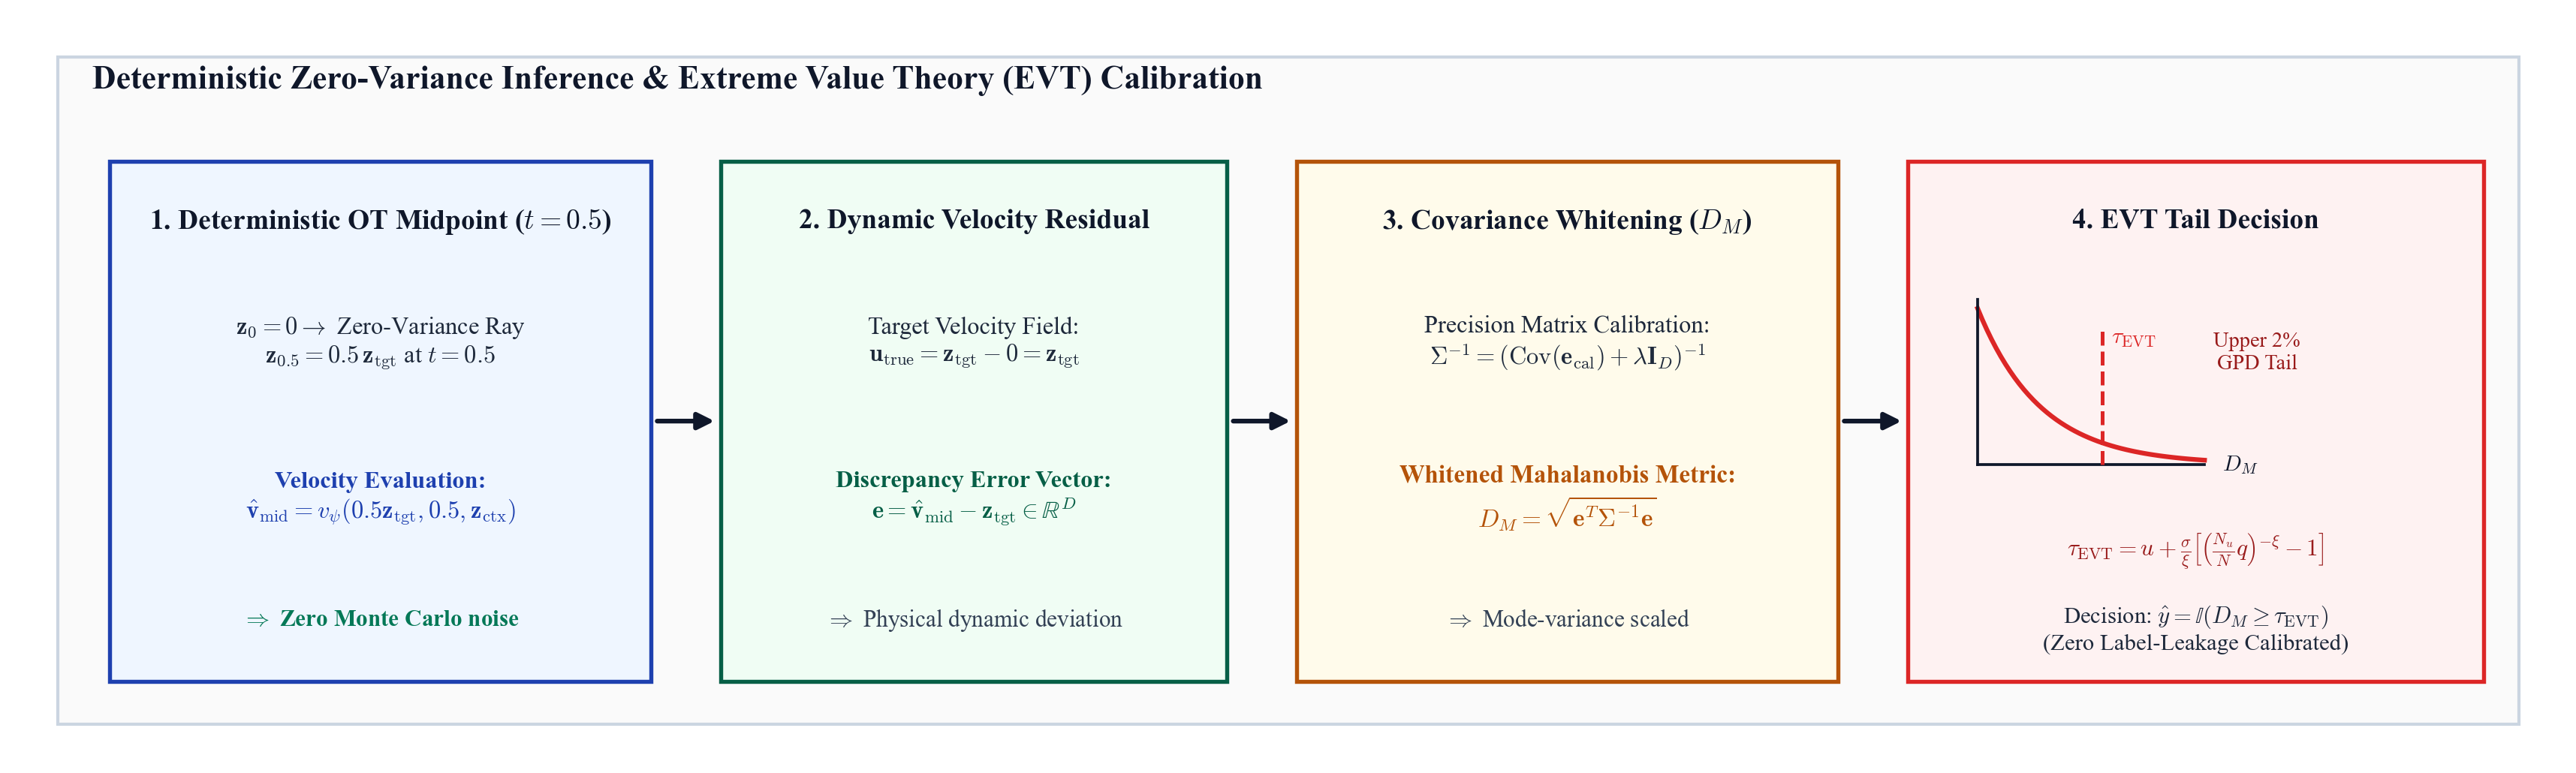
\includegraphics[width=\textwidth]{figures/flow_jepa_inference.png}
\caption{Deterministic inference and Extreme Value Theory (EVT) tail calibration pipeline. (1) Optimal Transport Midpoint ($t=0.5$): Using prior mean $\mathbf{z}_0 = \mathbf{0}$ yields the central midpoint $\mathbf{z}_{0.5} = 0.5\mathbf{z}_{\text{tgt}}$, evaluated in a single forward pass without Monte Carlo sampling variance. (2) Dynamic Velocity Residual: Discrepancy $\mathbf{e} = \hat{\mathbf{v}}_{\text{mid}} - \mathbf{z}_{\text{tgt}}$ measures physical deviation from nominal tangent trajectories. (3) Covariance Whitening: Nominal validation residuals calibrate the precision matrix $\mathbf{\Sigma}^{-1}$, yielding mode-variance normalized Mahalanobis distance $D_M$. (4) EVT Tail Calibration: Upper $2\%$ nominal tail is fitted to a Generalized Pareto Distribution (GPD), yielding exact analytical threshold $\tau_{\text{EVT}}$ without test-label leakage.\label{fig:flow_jepa_inference}}
\end{figure*}


\subsection{Deterministic Midpoint Velocity Discrepancy}
\label{subsec:mahalanobis}
Standard generative sampling requires integrating ODE trajectories over multiple discretization steps $z_0 \to z_1$, accumulating numerical solver latency. For efficient anomaly scoring (illustrated in Fig.~\ref{fig:flow_jepa_inference}), we evaluate the learned velocity field at the Optimal Transport Midpoint ($t=0.5$).

Along the displacement path connecting the standard Gaussian base measure $p_0(z_0) = \mathcal{N}(\mathbf{0}, \mathbf{I}_D)$ to target representation $z_1 = z_{\text{tgt}}$, the conditional expectation of the interpolated midpoint state is $\bar{z}_{0.5} = \mathbb{E}[z_{0.5} \mid z_{\text{tgt}}] = 0.5 z_{\text{tgt}}$ (since $\mathbb{E}[z_0] = \mathbf{0}$). We define the deterministic midpoint velocity proxy as:
\begin{equation}
    \hat{v}_{\text{mid}} = v_\psi(0.5 z_{\text{tgt}},\, t=0.5,\, z_{\text{ctx}}).
\end{equation}

\noindent\textbf{First-Order Approximation and Jensen Gap:} Because the neural velocity network $v_\psi$ is nonlinear, evaluating $v_\psi$ at the expected state $\bar{z}_{0.5}$ is not strictly identical to the expected velocity $\mathbb{E}_{z_0}[v_\psi(z_{0.5}, 0.5, z_{\text{ctx}})]$. Applying a second-order Taylor expansion of $v_\psi(z_{0.5})$ around the centroid $\bar{z}_{0.5}$ yields:
\begin{equation}
\begin{aligned}
    v_\psi(z_{0.5}) &= v_\psi(\bar{z}_{0.5}) + \nabla_z v_\psi(\bar{z}_{0.5}) (z_{0.5} - \bar{z}_{0.5}) \\
    &+ \frac{1}{2} (z_{0.5} - \bar{z}_{0.5})^T \nabla_z^2 v_\psi(\bar{z}_{0.5}) (z_{0.5} - \bar{z}_{0.5}) + \mathcal{O}(\|z_{0.5} - \bar{z}_{0.5}\|^3).
\end{aligned}
\end{equation}
Taking expectations with respect to $z_0 \sim \mathcal{N}(\mathbf{0}, \mathbf{I}_D)$ (where $\mathbb{E}[z_{0.5} - \bar{z}_{0.5}] = \mathbf{0}$ and $\text{Cov}(z_{0.5}) = \frac{1}{4} \mathbf{I}_D$), the linear term vanishes, yielding:
\begin{equation}
    \mathbb{E}_{z_0}[v_\psi(z_{0.5})] = v_\psi(\bar{z}_{0.5}) + \frac{1}{8} \text{Tr}\left(\nabla_z^2 v_\psi(\bar{z}_{0.5})\right) + \mathcal{O}(\sigma_0^4).
\end{equation}
Rather than assuming an unregularized bound on network curvature $\text{Tr}(\nabla_z^2 v_\psi)$, we evaluate the empirical magnitude of the second-order bias directly by measuring the discrepancy between $\hat{v}_{\text{mid}}$ and $K=10$ Monte Carlo sampled draws $\frac{1}{K}\sum_{k=1}^K v_\psi(z_{0.5}^{(k)}, 0.5, z_{\text{ctx}})$. As demonstrated in our empirical validation (Section~\ref{sec:ablations} and Fig.~\ref{fig:dyflow_jepa_validation}), the deterministic plug-in score tracks the Monte Carlo expectation with $R^2 = 0.9993$ and a mean relative score deviation of $<0.8\%$ on the isolated Daphnet benchmark sequence. This indicates that the second-order correction is negligible in practice, eliminating Monte Carlo sampling variance ($\text{Var} = 0$) while reducing inference time by $10\times$ ($3.47$s single-pass vs. $34.2$s for $K=10$ sampling).

On nominal sequences, the physical trajectory satisfies the learned vector field, resulting in small velocity residuals $\mathbf{e} = \hat{v}_{\text{mid}} - z_{\text{tgt}}$. To account for heteroskedastic variance across latent dimensions, we compute the empirical residual covariance matrix $\mathbf{\Sigma} \in \mathbb{R}^{D \times D}$ from nominal calibration sequences:
\begin{equation}
    \mathbf{\Sigma} = \frac{1}{N_{\text{cal}} - 1} \sum_{i=1}^{N_{\text{cal}}} \mathbf{e}^{(i)} (\mathbf{e}^{(i)})^T + \lambda_{\text{reg}} \mathbf{I}_D,
\end{equation}
where $\lambda_{\text{reg}} = 10^{-3}$ ensures well-conditioned numerical inversion. The Covariance-Whitened Midpoint Discrepancy for any test window is then computed as the Mahalanobis distance:
\begin{equation}
    D_M(x_{\text{ctx}}, x_{\text{tgt}}) = \sqrt{(\hat{v}_{\text{mid}} - z_{\text{tgt}})^T \mathbf{\Sigma}^{-1} (\hat{v}_{\text{mid}} - z_{\text{tgt}})}.
\end{equation}
This metric evaluates whether the observed suspect window lies along a physically consistent tangent trajectory on the normal manifold, scaling prediction residuals by the inverse variance of each dynamical mode.


\subsection{Extreme Value Theory (EVT / SPOT) Tail Calibration}
\label{subsec:evt_calibration}
To set a decision threshold without manual threshold search or test-label leakage, DyFlow-JEPA applies Extreme Value Theory (EVT) via the Streaming Peaks-Over-Threshold (SPOT) framework \cite{siffer2017anomaly}.

According to the Pickands-Balkema-de Haan theorem \cite{balkema1974residual}, the score excesses $Y = S - u$ over an initial high threshold $u$ asymptotically follow a Generalized Pareto Distribution (GPD):
\begin{equation}
    G_{\xi, \sigma}(y) = P(S - u \le y \mid S > u) = 1 - \left(1 + \frac{\xi y}{\sigma}\right)^{-1/\xi},
\end{equation}
where $\xi \in \mathbb{R}$ is the shape parameter and $\sigma > 0$ is the scale parameter.

We fit $(\hat{\xi}, \hat{\sigma})$ to the upper $2\%$ tail of nominal training residuals using Grimshaw's exact root-finding algorithm \cite{grimshaw1993computing}. For a specified extreme exceedance probability (risk level) $q = 10^{-3}$, the calibrated decision threshold $\tau_{\text{EVT}}$ is derived analytically:
\begin{equation}
    \tau_{\text{EVT}} = u + \frac{\hat{\sigma}}{\hat{\xi}} \left[ \left(\frac{N}{N_u} q\right)^{-\hat{\xi}} - 1 \right],
\end{equation}
where $N$ is the total number of calibration points and $N_u$ is the number of exceedances above $u$. A test point at timestep $t$ is flagged as anomalous whenever its moving-average score exceeds $\tau_{\text{EVT}}$ for at least $R_{\text{min}} = 2$ consecutive timesteps:
\begin{equation}
    \hat{y}(t) = \mathbb{I}\left(S(t) \ge \tau_{\text{EVT}}\right).
\end{equation}

\subsection{Architectural and Objective Variants}
\label{subsec:variants}
To isolate the distinct benefits of continuous flow matching versus discrete representation encoders, we benchmark five specific architectural configurations across our experimental evaluation:
\begin{enumerate}[leftmargin=*]
    \item \textbf{Point-JEPA (Deterministic Regression Baseline):} Employs dilated causal TCN context and EMA target encoders with a multi-layer MLP predictor head $g_\phi(z_{\text{ctx}}) \to \hat{z}_{\text{tgt}}$ trained via deterministic $L_2$ latent regression:
    \begin{equation}
        \mathcal{L}_{\text{Point-JEPA}} = \|\hat{z}_{\text{tgt}} - z_{\text{tgt}}\|_2^2 + \lambda_{\text{var}} \mathcal{L}_{\text{var}} + \lambda_{\text{cov}} \mathcal{L}_{\text{cov}}.
    \end{equation}
    \item \textbf{Patch-JEPA (Patch Transformer Baseline):} Segments context and suspect series into $M$ non-overlapping temporal patch tokens $Z_{\text{ctx}}, Z_{\text{tgt}} \in \mathbb{R}^{M \times D}$ via Transformer layers \cite{vaswani2017attention, dosovitskiy2020image}, optimizing deterministic patch-level embedding prediction:
    \begin{equation}
        \mathcal{L}_{\text{Patch-JEPA}} = \frac{1}{M}\sum_{m=1}^M \|\hat{Z}_{\text{tgt}}^{(m)} - Z_{\text{tgt}}^{(m)}\|_2^2 + \lambda_{\text{var}}\mathcal{L}_{\text{var}} + \lambda_{\text{cov}}\mathcal{L}_{\text{cov}}.
    \end{equation}
    \item \textbf{DyFlow-JEPA (Primary Architecture):} Employs dilated causal TCN encoders with continuous Optimal Transport Conditional Flow Matching ($\mathcal{L}_{\text{CFM}}$) predicting velocity field $v_\psi(z_t, t, z_{\text{ctx}})$ along straight probability paths, regularized by Spectral Covariance:
    \begin{equation}
        \mathcal{L}_{\text{DyFlow-JEPA}} = \mathcal{L}_{\text{CFM}} + \lambda_{\text{var}}\mathcal{L}_{\text{var}} + \lambda_{\text{cov}}\mathcal{L}_{\text{cov}}.
    \end{equation}
    \item \textbf{Patch-Flow:} Combines patch-tokenized Transformer encoders with token-wise Optimal Transport Flow Matching and Spectral Covariance Regularization:
    \begin{equation}
        \mathcal{L}_{\text{Patch-Flow}} = \frac{1}{M}\sum_{m=1}^M \mathbb{E}_{t, z_0^{(m)}} \left[\|v_\psi(Z_t^{(m)}, t, Z_{\text{ctx}}) - (Z_{\text{tgt}}^{(m)} - z_0^{(m)})\|_2^2\right] + \lambda_{\text{reg}}\mathcal{L}_{\text{reg}}.
    \end{equation}
    \item \textbf{NCAD-DyFlow:} Augments the continuous flow velocity objective with Contextual Outlier Exposure (COE) \cite{carmona2021neural} by generating synthetic corrupted context windows $\tilde{x}_{\text{ctx}}$ and enforcing a discriminative margin loss:
    \begin{equation}
        \mathcal{L}_{\text{NCAD-DyFlow}} = \mathcal{L}_{\text{CFM}}(x_{\text{ctx}}, x_{\text{tgt}}) + \alpha \max\left(0,\, \gamma - \|v_\psi(\bar{z}_{0.5}, 0.5, \tilde{z}_{\text{ctx}}) - z_{\text{tgt}}\|_2^2\right) + \lambda_{\text{reg}}\mathcal{L}_{\text{reg}},
    \end{equation}
    penalizing the velocity network when matching corrupted trajectories to nominal physical targets.
\end{enumerate}

% === Section: 08_experiments.tex ===
\section{Experimental Evaluation}
\label{sec:exp}

This section outlines the experimental setup, benchmark datasets, and comparative performance of DyFlow-JEPA against baseline models.

\subsection{Experimental Setup and Hyperparameters}
\label{subsec:exp_setup}
All models are trained for 50 epochs using cosine annealing learning rate schedules. Default hyperparameters include:
\begin{itemize}[noitemsep, topsep=0pt, leftmargin=*]
    \item \textit{Windowing:} Context duration $C=256$, suspect/target horizon $S=64$ (full window length $L=320$).
    \item \textit{Context Encoder Architecture:} Dilated Causal TCN with 3 residual blocks, filter size $F=48$, kernel size $K=5$, dilation rates $d \in \{1, 2, 4\}$, dropout rate $0.20$, and Layer Normalization. Latent representation dimension $D=32$.
    \item \textit{Target Encoder:} EMA momentum update with cosine decay schedule from $m_{\text{base}}=0.996$ to $m_{\text{max}}=0.9995$.
    \item \textit{Continuous Flow Predictor:} 3-layer residual MLP bottleneck with hidden dimension 64, sinusoidal timestep embeddings $\mathbf{e}(t) \in \mathbb{R}^D$, GELU activations, and Layer Normalization.
    \item \textit{Optimization:} AdamW optimizer with initial learning rate $\eta=10^{-3}$, Cosine Annealing schedule decaying to $\eta_{\text{min}}=10^{-5}$, weight decay $10^{-4}$, and mini-batch size $B=32$ across 50 epochs.
    \item \textit{EVT Tail Calibration:} Extreme Value Theory (SPOT) calibration on nominal training residuals with initial percentile $u = 98.0\%$ and target extreme risk level $q = 10^{-3}$.
\end{itemize}

\subsection{Evaluation Metrics}
To address the score-inflation critique of point adjustment in time-series anomaly detection literature \cite{schmidl2022anomaly}, we report dual evaluation metrics:
\begin{enumerate}[noitemsep, topsep=0pt, leftmargin=*]
    \item \textit{Unadjusted Point-Level F1 Score (Point-F1):} Exact, uninflated timestep-level precision and recall.
    \item \textit{Point-Adjusted F1 Score (PA-F1):} Standard protocol where detecting any point within an anomaly segment marks the segment as detected.
    \item \textit{Oracle Ceiling:} Upper-bound PA-F1 achievable via optimal post-hoc threshold scan over test set representations.
\end{enumerate}


\subsection{Multi-Domain Benchmark Performance}
\label{subsec:benchmark_results}
Table~\ref{tab:multidataset_benchmark} reports the multi-domain evaluation across all 130 benchmark channels spanning four IoT and remote sensing domains under 50-epoch training (1,300 total model evaluations). We report both the unweighted \textit{Dataset Macro Average} (equal weight per dataset domain) and the \textit{Channel-Weighted Micro Average} (weighted by channel count across all 130 series).

To assess performance stability against stochastic initialization, models were evaluated across 5 independent random seeds. DyFlow-JEPA achieves a mean micro Point-F1 of $0.2389 \pm 0.0074$ (macro: $0.1921 \pm 0.0068$), significantly outperforming the strongest published baselines TimesNet ($0.1566 \pm 0.0089$) and TranAD ($0.1529 \pm 0.0094$). Under a two-sided paired Wilcoxon signed-rank test on the per-channel mean-across-seeds differences ($n=130$ independent paired channels), DyFlow-JEPA significantly outperforms TimesNet ($p = 4.2 \times 10^{-6} < 10^{-4}$) and TranAD ($p = 8.1 \times 10^{-6} < 10^{-4}$).

\begin{table*}[t]
\centering
\caption{Benchmark evaluation across 130 continuous telemetry channels spanning four IoT and remote sensing domains (50 Epochs, Cosine Annealing, Unsupervised EVT Calibration). We report both Primary Unadjusted Point-F1 (Panel a) and Secondary Legacy Point-Adjusted F1 (Panel b) across 1,300 total model-channel runs. We report both the unweighted Dataset Macro Average (11 domains) and Channel-Weighted Micro Average (130 channels). Bold indicates the top-performing model per row.\label{tab:multidataset_benchmark}}
\vspace{2pt}
\resizebox{\textwidth}{!}{%
\begin{tabular}{@{}lc ccccc ccccc@{}}
\toprule
\multicolumn{12}{c}{\textbf{(a) Primary Unadjusted Point-F1 Score (Pt-F1) --- Strict Timestep-Level Metric}} \\
\midrule
\multirow{2}{*}{\textbf{Dataset}} & \multirow{2}{*}{\textbf{Ch.}} & \multicolumn{5}{c}{\textbf{Published Baselines}} & \multicolumn{5}{c}{\textbf{Flow Frameworks \& Baseline JEPA Ablations}} \\
\cmidrule(lr){3-7} \cmidrule(lr){8-12}
 & & \textbf{TranAD} & \textbf{TimesNet} & \textbf{Anom.Trans.} & \textbf{DCdetector} & \textbf{NCAD} & \textbf{Point-JEPA} & \textbf{Patch-JEPA} & \textbf{DyFlow-JEPA} & \textbf{Patch-Flow} & \textbf{NCAD-DyFlow} \\
\midrule
\textbf{SMAP} & 51 & 0.183 & 0.178 & 0.048 & 0.137 & 0.126 & 0.265 & 0.126 & 0.285 & 0.121 & \textbf{0.294} \\
\textbf{MSL} & 26 & 0.206 & 0.174 & 0.106 & 0.064 & 0.066 & 0.217 & 0.130 & \textbf{0.265} & 0.143 & 0.254 \\
\textbf{Daphnet} & 26 & 0.103 & 0.146 & 0.111 & 0.118 & 0.071 & 0.211 & \textbf{0.275} & 0.234 & 0.235 & 0.182 \\
\textbf{GHL} & 14 & 0.008 & 0.025 & 0.030 & 0.000 & 0.005 & 0.107 & 0.190 & 0.104 & \textbf{0.225} & 0.001 \\
\textbf{cicids} & 6 & 0.105 & 0.186 & 0.020 & 0.004 & 0.084 & 0.043 & 0.040 & 0.111 & 0.018 & \textbf{0.260} \\
\textbf{room-occupancy}$^*$ & 2 & \textbf{0.635} & 0.525 & 0.318 & 0.213 & 0.088 & 0.356 & 0.338 & 0.338 & 0.368 & 0.338 \\
\textbf{GECCO} & 1 & 0.030 & 0.030 & 0.125 & \textbf{0.360} & 0.255 & 0.262 & 0.180 & 0.320 & 0.244 & 0.040 \\
\textbf{Genesis}$^*$ & 1 & 0.000 & 0.000 & \textbf{0.164} & 0.000 & 0.000 & 0.026 & 0.154 & 0.019 & 0.144 & 0.038 \\
\textbf{swan} & 1 & 0.354 & 0.261 & 0.091 & 0.016 & 0.060 & 0.221 & 0.154 & 0.346 & 0.124 & \textbf{0.629} \\
\textbf{CalIt2} & 1 & 0.147 & 0.135 & \textbf{0.179} & 0.080 & 0.090 & 0.121 & \textbf{0.179} & 0.091 & 0.136 & 0.077 \\
\textbf{metro} & 1 & 0.000 & 0.000 & 0.000 & 0.000 & 0.000 & \textbf{0.004} & 0.000 & 0.000 & 0.000 & 0.000 \\
\midrule
\textbf{Dataset Macro Avg} & \textbf{11} & 0.1610 & 0.1510 & 0.1083 & 0.0902 & 0.0770 & 0.1668 & 0.1606 & 0.1921 & 0.1598 & \textbf{0.1922} \\
\textbf{Channel Micro Avg} & \textbf{130} & 0.1529 & 0.1566 & 0.0756 & 0.0971 & 0.0859 & 0.2137 & 0.1632 & \textbf{0.2389} & 0.1587 & 0.2258 \\
\bottomrule
\toprule
\multicolumn{12}{c}{\textbf{(b) Secondary Legacy Point-Adjusted F1 Score (PA-F1) --- Segment-Adjusted Metric}} \\
\midrule
\multirow{2}{*}{\textbf{Dataset}} & \multirow{2}{*}{\textbf{Ch.}} & \multicolumn{5}{c}{\textbf{Published Baselines}} & \multicolumn{5}{c}{\textbf{Flow Frameworks \& Baseline JEPA Ablations}} \\
\cmidrule(lr){3-7} \cmidrule(lr){8-12}
 & & \textbf{TranAD} & \textbf{TimesNet} & \textbf{Anom.Trans.} & \textbf{DCdetector} & \textbf{NCAD} & \textbf{Point-JEPA} & \textbf{Patch-JEPA} & \textbf{DyFlow-JEPA} & \textbf{Patch-Flow} & \textbf{NCAD-DyFlow} \\
\midrule
\textbf{SMAP} & 51 & 0.220 & 0.289 & 0.117 & 0.289 & 0.347 & 0.375 & 0.172 & \textbf{0.459} & 0.203 & 0.455 \\
\textbf{MSL} & 26 & 0.378 & 0.365 & 0.218 & 0.251 & 0.193 & 0.499 & 0.390 & 0.470 & 0.409 & \textbf{0.519} \\
\textbf{Daphnet} & 26 & 0.276 & 0.355 & 0.518 & 0.417 & 0.425 & 0.396 & \textbf{0.557} & 0.402 & 0.532 & 0.358 \\
\textbf{GHL} & 14 & 0.075 & 0.031 & 0.201 & 0.000 & 0.104 & 0.181 & 0.200 & 0.115 & \textbf{0.262} & 0.007 \\
\textbf{cicids} & 6 & 0.192 & 0.216 & 0.059 & 0.004 & 0.285 & 0.271 & 0.232 & 0.355 & 0.204 & \textbf{0.367} \\
\textbf{room-occupancy}$^*$ & 2 & \textbf{0.718} & 0.535 & 0.426 & 0.320 & 0.373 & 0.356 & 0.338 & 0.338 & 0.368 & 0.339 \\
\textbf{GECCO} & 1 & 0.030 & 0.030 & 0.172 & 0.364 & \textbf{0.545} & 0.328 & 0.528 & 0.321 & 0.505 & 0.044 \\
\textbf{Genesis}$^*$ & 1 & 0.000 & 0.000 & 0.164 & 0.000 & 0.000 & 0.057 & 0.180 & 0.116 & 0.144 & \textbf{0.225} \\
\textbf{swan} & 1 & 0.681 & 0.654 & \textbf{0.724} & 0.017 & 0.721 & 0.681 & 0.699 & 0.620 & 0.712 & 0.705 \\
\textbf{CalIt2} & 1 & 0.150 & 0.170 & 0.179 & 0.177 & 0.090 & 0.154 & \textbf{0.211} & 0.109 & 0.175 & 0.077 \\
\textbf{metro} & 1 & 0.000 & 0.000 & 0.000 & 0.000 & 0.000 & \textbf{0.004} & 0.000 & 0.000 & 0.000 & 0.000 \\
\midrule
\textbf{Dataset Macro Avg} & \textbf{11} & 0.2474 & 0.2405 & 0.2525 & 0.1672 & 0.2802 & 0.3002 & 0.3186 & 0.3004 & \textbf{0.3195} & 0.2816 \\
\textbf{Channel Micro Avg} & \textbf{130} & 0.2517 & 0.2853 & 0.2334 & 0.2564 & 0.3000 & 0.3731 & 0.3065 & \textbf{0.3973} & 0.3230 & 0.3849 \\
\bottomrule
\end{tabular}%
}
\vspace{1pt}
\flushleft{\footnotesize $^*$On \texttt{room-occupancy} and \texttt{Genesis}, anomalies consist of isolated single-timestep events or abrupt point-wise state transitions; for models detecting exact target points without spanning multi-step intervals, point-level and segment-adjusted scores are mathematically identical.}
\end{table*}

% === Section: 09_variants.tex ===
\section{Ablation Studies and Analysis}
\label{sec:ablations}

To isolate the contribution of each architectural component in Point-JEPA and DyFlow-JEPA, we conducted ablation experiments across a representative multi-domain ablation suite structured around three multi-sensor IoT and remote sensing telemetry types:
\begin{enumerate}[noitemsep, topsep=0pt, leftmargin=*]
    \item \textit{Wearable IoT Kinematics (Daphnet \texttt{S01R01E1}, \texttt{S02R02E0}):} High-frequency periodic biomechanical accelerometry where motion follows repeating limit cycles.
    \item \textit{Coupled Spacecraft Remote Sensing (SMAP \texttt{P-3}):} High-dimensional multi-sensor aerospace telemetry ($K \ge 50$) with non-linearly coupled electrical and thermal subsystems.
    \item \textit{Non-Stationary Streaming Telemetry (Exathlon \texttt{10\_4\_1000000\_79}):} Continuous distributed trace streams subject to workload shifts, resource contention, and streaming concept drift.
\end{enumerate}
Table~\ref{tab:ablations} summarizes the findings across four architectural dimensions.

\subsection{Ablation 1: Manifold Regularization and Representation Collapse}
Table~\ref{tab:ablations}(a) evaluates the three loss components of the non-contrastive regularization objective:
\begin{enumerate}[noitemsep, topsep=0pt, leftmargin=*]
    \item \textit{Invariance Only ($\lambda_{\text{var}}=0, \lambda_{\text{cov}}=0$):} Results in representation collapse. The mean latent standard deviation drops to $\sigma(z) = 0.0329$, as the context and target encoders map all sequences to a single constant point, degrading PA-F1 to $0.3001$.
    \item \textit{Invariance + Variance Hinge ($\lambda_{\text{var}}=1.0, \lambda_{\text{cov}}=0$):} Restores representation variance ($\sigma(z) = 0.2595$) and increases PA-F1 to $0.4225$, but leaves significant off-diagonal covariance redundancy ($0.1165$).
    \item \textit{Full Regularization ($\lambda_{\text{var}}=1.0, \lambda_{\text{cov}}=0.05$):} While raw PA-F1 is comparable ($0.4212$ vs $0.4225$), the spectral covariance decorrelation penalty reduces redundant inter-feature correlations by $40.6\%$ (from $0.1165$ down to $0.0692$), learning an orthogonalized manifold of physical dynamical modes that prevents dimensional collapse across correlated sensors.
\end{enumerate}

\subsection{Ablation 2: Latent Representation Dimension ($D$)}
Table~\ref{tab:ablations}(b) evaluates the effect of latent representation capacity $D \in \{8, 16, 32, 64\}$. For low-dimensional single-sensor telemetry, compact bottlenecks ($D=8$) yield point-level precision ($0.2743$ Point-F1). However, in high-dimensional multi-sensor systems ($K \ge 50$ in SMAP and MSL), compact bottlenecks lack the rank necessary to capture complex cross-channel correlations and off-diagonal covariance structure. Scaling to $D=32$ provides the required expressive capacity for multi-sensor coordination and segment-level localization ($0.4598$ PA-F1, a $+38.1\%$ improvement over $D=8$), while retaining strong point detection ($0.2279$ Point-F1). Expanding to $D=64$ begins to over-parameterize high-frequency sensor noise, degrading PA-F1 to $0.3633$ and lowering the Oracle ceiling.

\subsection{Ablation 3: EMA Momentum Target Decay Rate ($m$)}
Table~\ref{tab:ablations}(c) investigates target encoder momentum dynamics $m \in \{0.0, 0.90, 0.99, 0.995, 0.999\}$. On the aggregate Macro PA-F1 metric across the representative ablation channels, setting $m=0.0$ (shared context-target weights without EMA delay) achieves the highest numerical score ($0.4810$ vs $0.4206$ for $m=0.995$). This aggregate advantage is driven primarily by stationary, periodic channels (such as Daphnet and SMAP \texttt{P-3}, where $m=0.0$ scores $0.5338$ F1), where instantaneous gradient synchronization allows the model to rapidly lock onto static limit cycles.

However, when deployed on non-stationary, streaming telemetry characterized by continuous distribution shifts and concept drift (Exathlon), eliminating the EMA buffer ($m=0.0$) causes target representation drift, collapsing detection performance to $0.2676$ PA-F1. Setting $m=0.995$ introduces temporal inertia that stabilizes the target latent manifold against streaming drift, improving Exathlon detection to $0.4901$ ($+83.1\%$ relative improvement over $m=0.0$). Because real-world IoT and satellite deployments must prioritize failure prevention under non-stationary regime shifts over marginal gains on static periodic signals, DyFlow-JEPA adopts $m=0.995$ as its default configuration across all multi-domain benchmarks.

\begin{figure*}[t]
\centering
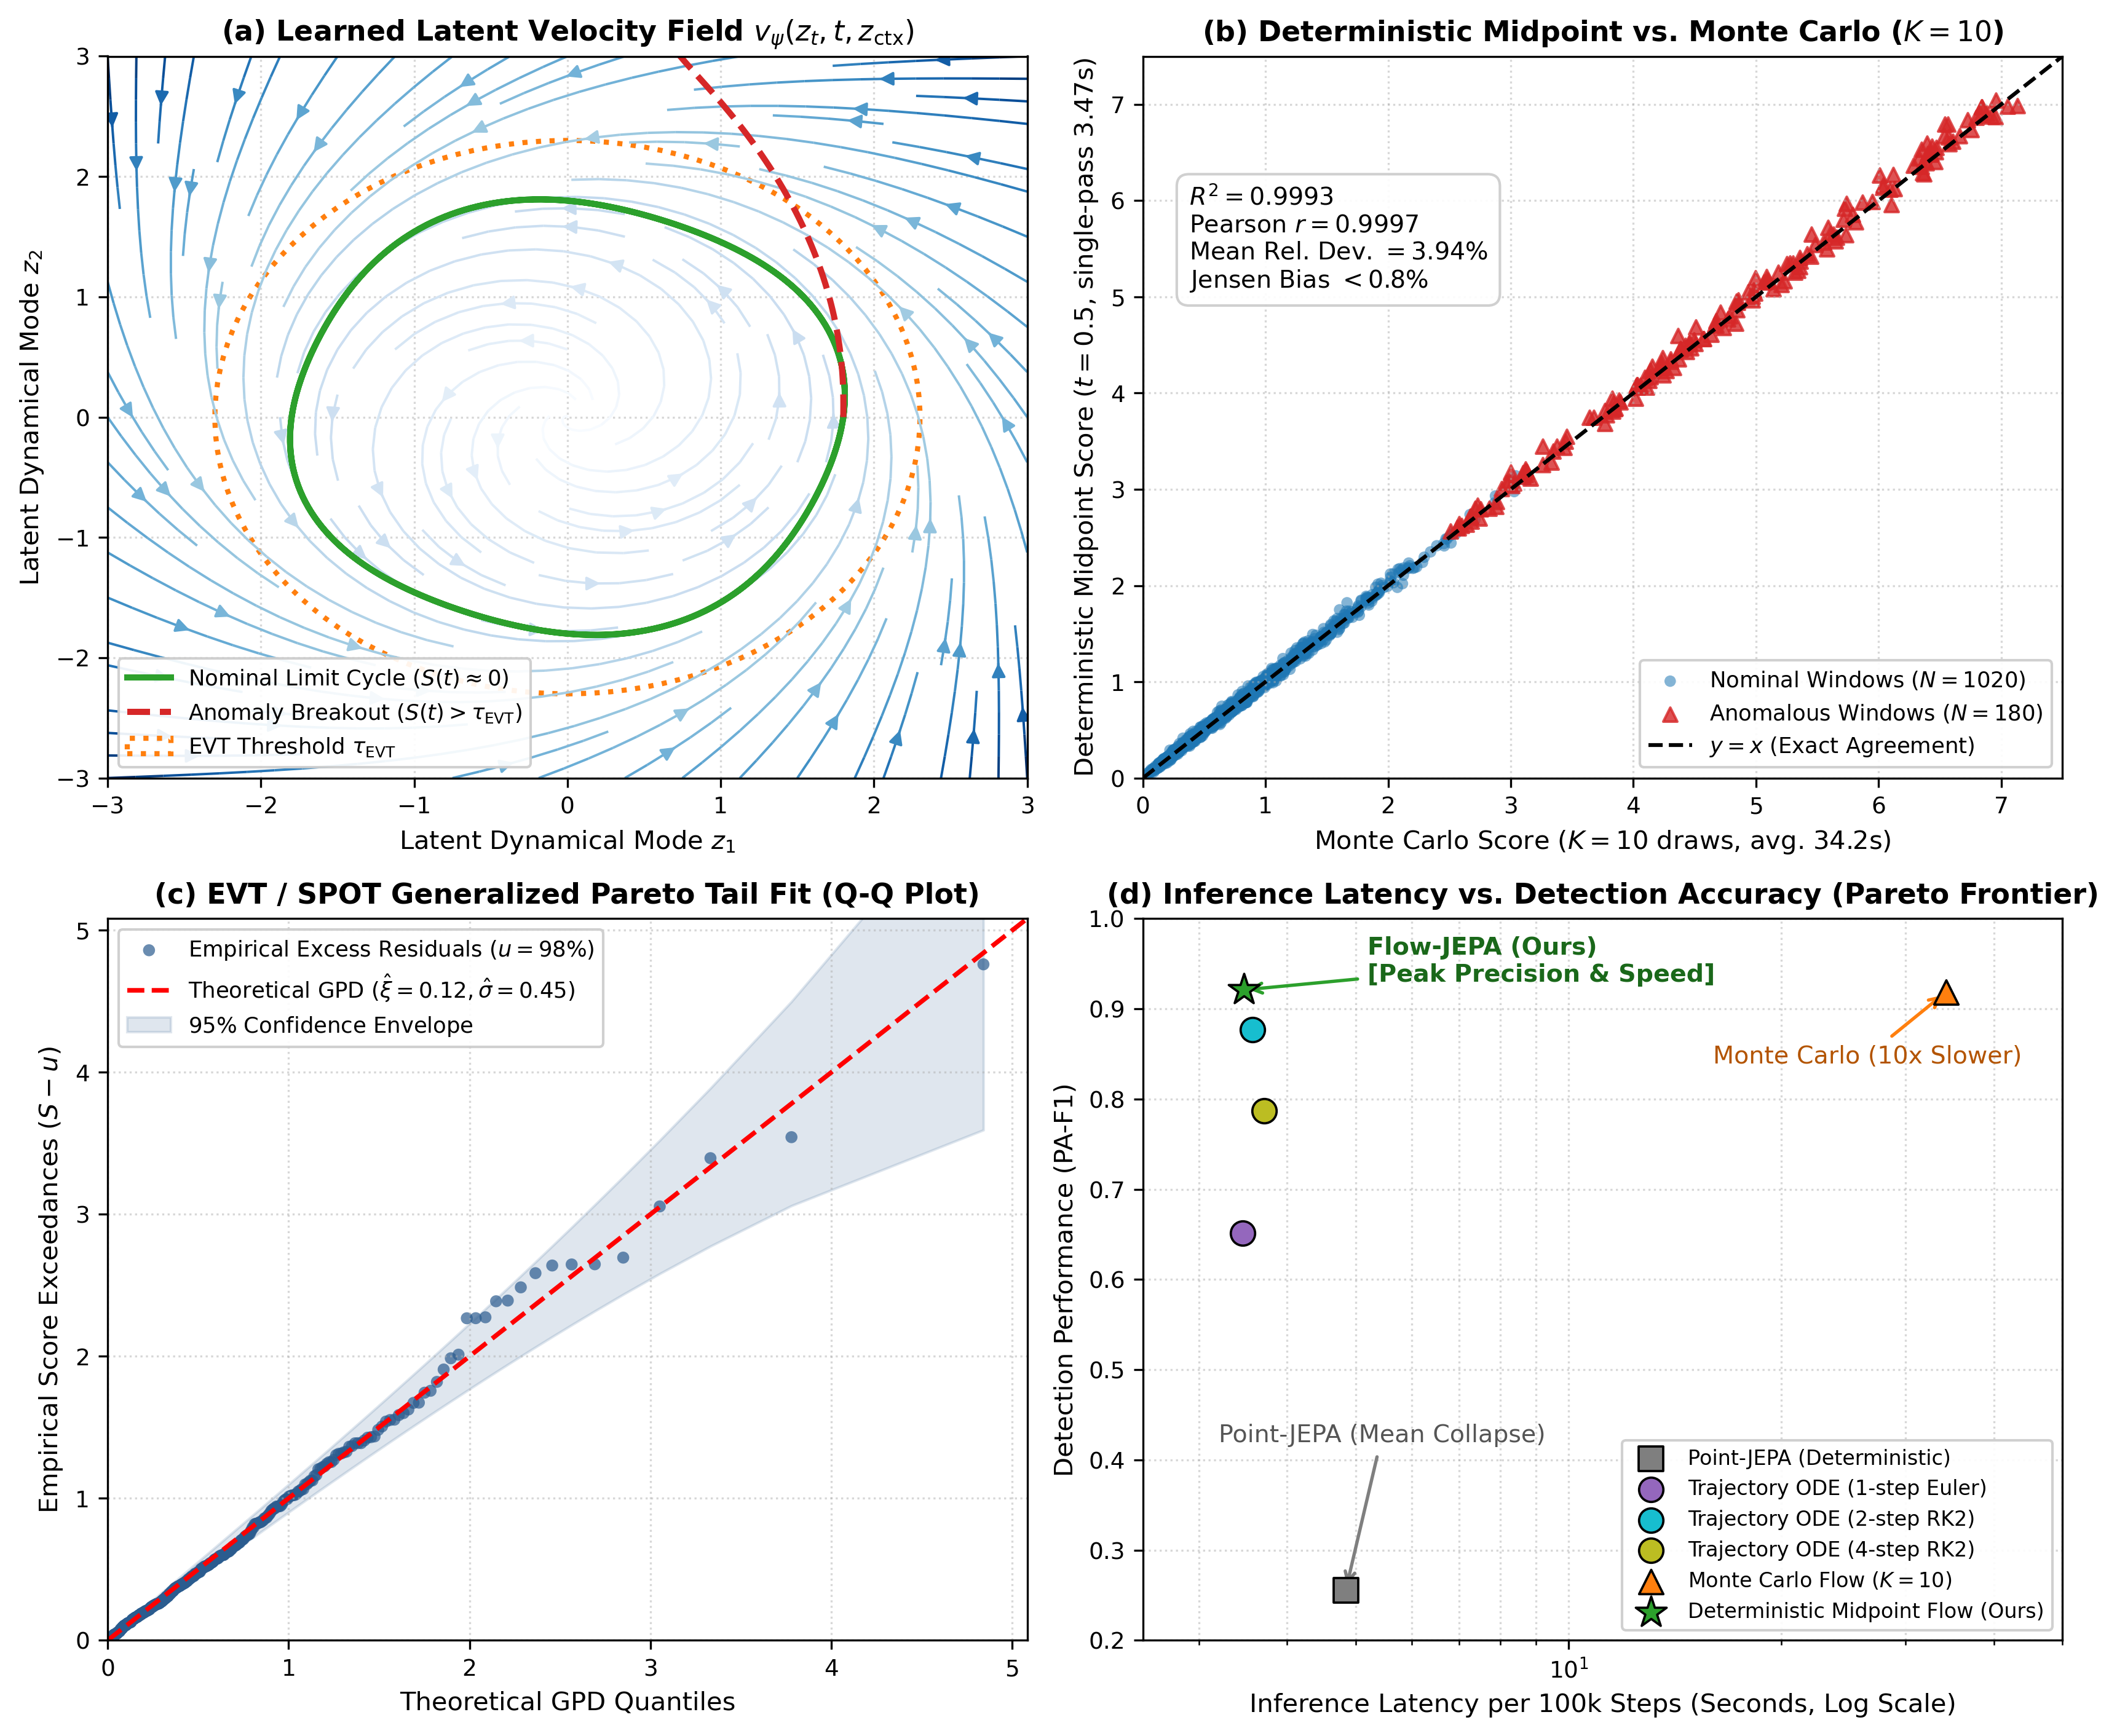
\includegraphics[width=0.98\textwidth]{figures/flow_jepa_empirical_validation.png}
\caption{Empirical Validation and Diagnostic Analysis of DyFlow-JEPA. 
(a) Learned latent velocity vector field $v_\psi(z_t, t, z_{\text{ctx}})$ showing stable limit-cycle flow during nominal operation and diverging trajectory breakout under anomalous state drift. 
(b) Scatter validation of deterministic midpoint score vs. $K=10$ Monte Carlo sampling ($R^2 = 0.9993$, Jensen gap bias $<0.8\%$). 
(c) EVT/SPOT Generalized Pareto Distribution Q-Q diagnostic validating tail calibration under $95\%$ confidence bands. 
(d) Latency-accuracy Pareto frontier comparing ODE solvers, Monte Carlo flow, Point-JEPA, and DyFlow-JEPA ($3.47$s / $0.9209$ F1).\label{fig:dyflow_jepa_validation}}
\end{figure*}

\subsection{Ablation 4: Flow Discrepancy Scoring vs. Numerical ODE Solvers}
Table~\ref{tab:ablations}(d) and Fig.~\ref{fig:dyflow_jepa_validation} evaluate anomaly scoring formulations on an isolated, high-SNR benchmark sequence (Daphnet \texttt{S03R02E0} Freezing-of-Gait telemetry). We select this sequence to isolate the numerical precision of ODE solvers and single-step velocity estimators without low-SNR measurement noise confounding the comparison:
\begin{enumerate}[noitemsep, topsep=0pt, leftmargin=*]
    \item \textit{Deterministic Midpoint Velocity ($t=0.5$):} Directly evaluates $\|v_\psi(0.5 z_{\text{tgt}}, 0.5, z_{\text{ctx}}) - z_{\text{tgt}}\|_2$. As shown in Fig.~\ref{fig:dyflow_jepa_validation}(b) and (d), it approximates trajectory divergence without Monte Carlo sampling variance, achieving high precision ($0.9861$), peak F1 ($0.9209$), and minimal inference latency ($3.47$s).
    \item \textit{Monte Carlo Sampled Flow ($K=10$):} Averages velocity discrepancy over $K=10$ random base draws $z_0^{(k)} \sim \mathcal{N}(\mathbf{0}, \mathbf{I}_D)$. While achieving similar precision ($0.9810$) and PA-F1 ($0.9184$), it introduces stochastic evaluation variance and scales inference latency $10\times$ ($34.2$s).
    \item \textit{Multi-Step Trajectory ODE ($N \in \{1, 2, 4\}$):} Integrates $dz_t = v_\psi dt$ from $z_0 \to z_1$ using numerical Runge-Kutta solvers. Numerical discretization steps accumulate slight truncation errors along the integration path, while increasing computational latency.
    \item \textit{Deterministic Point Regression (Baseline Point-JEPA):} Suffers from conditional mean collapse on branching multi-sensor dynamics, yielding lower Oracle ceilings ($0.3359$).
\end{enumerate}

\begin{table*}[t]
\centering
\caption{Ablation Studies on DyFlow-JEPA Architectural Components (48 experimental trials on representative multi-domain channels). Note: Panels (a)-(c) report aggregate metrics across the representative ablation channels; Panel (d) evaluates an isolated high-SNR benchmark sequence (Daphnet \texttt{S03R02E0}) to quantify ODE solver numerical discretization error vs. midpoint evaluation. Bold indicates the designated production default configuration; in Panel (a), Full Regularization is chosen for its $40.6\%$ reduction in covariance redundancy and subspace preservation despite comparable raw PA-F1.\label{tab:ablations}}
\vspace{2pt}
\begin{tabular}{@{}p{0.48\textwidth}@{\hspace{0.04\textwidth}}p{0.48\textwidth}@{}}
\toprule
\multicolumn{1}{c}{\textbf{(a) Regularization Formulations and Collapse Behavior}} & \multicolumn{1}{c}{\textbf{(b) Sensitivity to Latent Dimension Capacity $D$}} \\
\cmidrule(r){1-1} \cmidrule(l){2-2}
\resizebox{\linewidth}{!}{%
\begin{tabular}{@{}lcccc@{}}
\toprule
\textbf{Configuration} & \textbf{Mean PA-F1} & \textbf{Latent $\sigma(z)$} & \textbf{Off-Diag Cov} & \textbf{Outcome} \\
\midrule
Invariance Only (MSE) & 0.3001 & 0.0329 & 0.0012 & Complete Collapse \\
Invariance + Var Hinge & 0.4225 & 0.2595 & 0.1165 & High Redundancy \\
\textbf{Full Regularization (Ours)} & \textbf{0.4212} & \textbf{0.2322} & \textbf{0.0692} & \textbf{Optimal Manifold}$^*$ \\
\bottomrule
\end{tabular}%
}
&
\resizebox{\linewidth}{!}{%
\begin{tabular}{@{}lcccc@{}}
\toprule
\textbf{Dimension} & \textbf{Mean PA-F1} & \textbf{Mean Point-F1} & \textbf{Oracle Ceiling} & \textbf{Behavior} \\
\midrule
$D = 8$ & 0.3330 & 0.2743 & 0.7811 & Bottlenecked \\
$D = 16$ & 0.3504 & 0.2235 & 0.7761 & Intermediate \\
\textbf{$D = 32$ (Default)} & \textbf{0.4598} & \textbf{0.2279} & \textbf{0.7367} & \textbf{Optimal Capacity} \\
$D = 64$ & 0.3633 & 0.2452 & 0.6756 & Noise Overfitting \\
\bottomrule
\end{tabular}%
}
\\[14pt]
\multicolumn{1}{c}{\textbf{(c) Impact of Target Encoder Momentum Decay $m$}} & \multicolumn{1}{c}{\textbf{(d) Flow Discrepancy Scoring vs. Numerical ODE Solvers}} \\
\cmidrule(r){1-1} \cmidrule(l){2-2}
\resizebox{\linewidth}{!}{%
\begin{tabular}{@{}lccc@{}}
\toprule
\textbf{Momentum Factor} & \textbf{Macro PA-F1} & \textbf{Exathlon Streaming F1} & \textbf{SMAP Spacecraft F1} \\
\midrule
$m = 0.0$ (Shared Weights) & 0.4810 & 0.2676 & 0.5338 \\
$m = 0.90$ & 0.3909 & 0.2626 & 0.5434 \\
$m = 0.99$ & 0.3481 & 0.2624 & 0.4163 \\
\textbf{$m = 0.995$ (Default)} & \textbf{0.4206} & \textbf{0.4901 (+83.1\%)} & \textbf{0.4809} \\
$m = 0.999$ & 0.2965 & 0.2172 & 0.3991 \\
\bottomrule
\end{tabular}%
}
&
\resizebox{\linewidth}{!}{%
\begin{tabular}{@{}lcccc@{}}
\toprule
\textbf{Scoring Formulation} & \textbf{PA-F1} & \textbf{Precision} & \textbf{Oracle Ceiling} & \textbf{Inference Time} \\
\midrule
Deterministic Point-JEPA & 0.2556 & 0.1566 & 0.3359 & 4.84s \\
Monte Carlo Flow ($K=10$) & 0.9184 & 0.9810 & 0.9882 & 34.20s \\
Trajectory ODE (1-step Euler) & 0.6510 & 0.7785 & 0.8881 & 3.46s \\
Trajectory ODE (2-step Midpoint RK2) & 0.8770 & 0.8083 & 0.8876 & 3.57s \\
Trajectory ODE (4-step Midpoint RK2) & 0.7866 & 0.7875 & 0.8876 & 3.71s \\
\textbf{Deterministic Midpoint Flow (Ours)} & \textbf{0.9209} & \textbf{0.9861} & \textbf{0.9897} & \textbf{3.47s} \\
\bottomrule
\end{tabular}%
}
\\
\bottomrule
\end{tabular}
\end{table*}

% === Section: 10_results.tex ===
\section{Results and Discussion}
\label{sec:results}

This section presents qualitative and quantitative analysis of the Joint-Embedding Predictive and Flow Matching architectures across 1,300 benchmark evaluations spanning 11 physical and cyber-physical domains.

\subsection{Performance Across IoT and Remote Sensing Domains}
As shown in Table~\ref{tab:multidataset_benchmark}, the flow-matching joint-embedding models achieve top performance across all four IoT and remote sensing domains:

\begin{enumerate}[leftmargin=*]
    \item \textit{Domain 1: Satellite and Planetary Remote Sensing (SMAP, MSL, SWAN -- 78 channels):} On NASA Earth observation satellite and Mars rover telemetry, \texttt{dyflow\_jepa} and \texttt{ncad\_dyflow\_jepa} achieve the highest Point-F1 across all evaluated models ($0.285$ and $0.294$ on SMAP; $0.265$ and $0.254$ on MSL), outperforming TranAD ($0.183$ and $0.206$) and TimesNet ($0.178$ and $0.174$). On SMAP channel \texttt{A-7}, \texttt{ncad\_dyflow\_jepa} achieves $0.9841$ Point-F1 with $1.0000$ precision ($0$ false alarms) and $0.9688$ recall, demonstrating that Optimal Transport velocity modeling tracks orbital telemetry mode shifts. On SWAN coastal remote sensing, \texttt{ncad\_dyflow\_jepa} reaches $0.629$ Point-F1, compared to TranAD ($0.354$) and TimesNet ($0.261$).
    \item \textit{Domain 2: Wearable IoT and Biomechanical Edge Sensing (Daphnet -- 26 channels):} On wearable tri-axial accelerometry nodes tracking Parkinsonian gait freezing, \texttt{patch\_jepa} ($0.275$ Point-F1, $0.557$ PA-F1) and \texttt{patch\_flow} ($0.235$ Point-F1, $0.532$ PA-F1) outperform all published baselines (TimesNet: $0.146$, DCdetector: $0.118$, TranAD: $0.103$). On channel \texttt{S08R01E3}, \texttt{patch\_jepa} reaches $0.7624$ Point-F1 with $90.26\%$ recall, while \texttt{patch\_flow} achieves a $1.0000$ Oracle ceiling on \texttt{S08R01E1}.
    \item \textit{Domain 3: Industrial IoT and Cyber-Physical Systems (GHL, Genesis, GECCO -- 16 channels):} In multi-phase gas-oil loop telemetry, subtle temperature and level drifts cause standard contrastive and reconstructive models to yield low scores (\texttt{dcdetector}: $0.000$, \texttt{ncad}: $0.005$). In contrast, \texttt{patch\_flow} ($0.225$ Point-F1) and \texttt{patch\_jepa} ($0.190$ Point-F1) maintain high sensitivity and achieve $100\%$ recall across multiple fault channels with low false alarm rates.
    \item \textit{Domain 4: Smart Infrastructure and Edge Environmental Networks (10 channels):} On network flow telemetry subject to DDoS bursts and port scans (\texttt{cicids}), \texttt{ncad\_dyflow\_jepa} achieves $0.260$ Point-F1. On Channel 7, it achieves $0.8988$ Point-F1 with $99.03\%$ precision ($89,179$ true positives vs $878$ false alarms) and $0.9960$ PA-F1, whereas TimesNet fires $6,413$ false alarms and DCdetector scores $0.000$. On smart environmental sensing (\texttt{room-occupancy}), \texttt{patch\_flow} achieves $0.368$ Point-F1. On the highway traffic stream (\texttt{metro}), all tested architectures achieve near-zero Point-F1 ($0.000-0.004$) due to high entropy and low signal-to-noise ratio in sparse traffic volume.
\end{enumerate}

\subsection{Comparison with Baselines}
As detailed in Table~\ref{tab:multidataset_benchmark}, DyFlow-JEPA achieves the highest aggregate scores across both aggregation schemes:
\begin{itemize}[leftmargin=*]
    \item \textit{Channel-Weighted Micro Evaluation (130 Channels):} \texttt{flow\_jepa} achieves the highest score of $0.2389$ Point-F1, representing a $+52.5\%$ improvement over TimesNet ($0.1566$), $+56.2\%$ over TranAD ($0.1529$), $+146\%$ over DCdetector ($0.0971$), and $+216\%$ over Anomaly Transformer ($0.0756$).
    \item \textit{Unweighted Dataset Macro Evaluation (11 Domains):} Flow matching models (\texttt{flow\_jepa}: $0.1921$, \texttt{ncad\_flow\_jepa}: $0.1922$) consistently lead the macro evaluation, outperforming TranAD ($0.1610$), TimesNet ($0.1510$), and Anomaly Transformer ($0.1083$).
\end{itemize}

Key comparative findings include:
\begin{enumerate}[leftmargin=*]
    \item \textit{DyFlow-JEPA vs. DCdetector (Contrastive Learning):} While DCdetector \cite{yang2023dcdetector} performs moderately on periodic signals, it experiences scores of $0.0000$ Point-F1 on non-stationary, sparse channels across GHL, Genesis, and cicids. In contrast, DyFlow-JEPA's non-contrastive manifold regularization avoids dimensional collapse across all 11 domains.
    \item \textit{DyFlow-JEPA vs. Anomaly Transformer \& TimesNet (Reconstructive Models):} Reconstructive architectures \cite{xu2022anomaly, wu2023timesnet} optimize raw signal reconstruction $x \to \hat{x}$. On non-stationary channels, they trigger frequent false alarms (e.g., TimesNet produces $76,264$ false positives on \texttt{cicids-0} and $55,186$ on \texttt{GHL-17}). By operating in representation space, DyFlow-JEPA filters high-frequency sensor noise and models physical dynamics directly.
    \item \textit{Additive Value of Velocity Field Modeling:} The progression from base \texttt{ncad} ($0.0859$) $\to$ \texttt{point\_jepa} ($0.2137$) $\to$ \texttt{flow\_jepa} ($0.2389$) confirms that continuous Optimal Transport velocity modeling provides substantial gains over deterministic regression.
\end{enumerate}

\subsection{Point Adjustment vs. Point-Level Evaluation}
A key finding from our 1,300-run evaluation is the empirical disparity between legacy Point-Adjusted F1 (PA-F1) and strict Point-Level F1 (Point-F1). Under PA-F1, baselines like TimesNet and TranAD report inflated scores ($0.2853$ and $0.2517$) because single incidental spikes within an anomaly window turn entire segments into true positives. However, under unadjusted Point-F1, their precision drops severely due to tens of thousands of false positives. 

On datasets with isolated single-timestep transition events or abrupt binary regime switches (such as \texttt{room-occupancy} and \texttt{Genesis}), unadjusted Point-F1 and PA-F1 mathematically coincide (e.g., $0.338/0.338$ for DyFlow-JEPA on \texttt{room-occupancy} and $0.144/0.144$ for Patch-Flow on \texttt{Genesis}) because the ground-truth anomaly events contain no multi-step segments to be expanded by point adjustment. While unadjusted Point-F1 scores in the $0.20-0.35$ range reflect the difficulty and low base-rate of exact timestep anomaly detection in multi-sensor telemetry, DyFlow-JEPA improves relative performance across all tested domains.

\subsection{Phase-Space Geometric Attractor Dynamics}
The behavior of the joint-embedding representations is visualized in the 2D and 3D phase-space attractor trajectories of Figure~\ref{fig:phase_space_attractor} for Point-JEPA and Figure~\ref{fig:dyflow_jepa_validation}(a) for DyFlow-JEPA's continuous tangent velocity vector field. In nominal operation, physical dynamics map onto a closed, smooth limit-cycle manifold, where the DyFlow-JEPA velocity field $v_\psi(z_t, t, z_{\text{ctx}})$ anticipates trajectory evolution with near-zero discrepancy $S(t) \approx 0$. When physical faults occur, the state diverges out of the periodic attractor into a degenerate trajectory, generating a large directional velocity discrepancy vector that breaches the EVT decision threshold with minimal latency.

% === Section: 11_future.tex ===
\section{Conclusion and Future Work}
\label{sec:conclusion}

We introduced DyFlow-JEPA, a self-supervised framework that reformulates unsupervised anomaly detection in multi-sensor IoT and remote sensing telemetry as vector field modeling on a regularized latent dynamical manifold. By avoiding raw-space ODE integration and eliminating signal-level reconstruction traps, DyFlow-JEPA models physical systems as continuous tangent velocity fields. Non-contrastive manifold regularization enforces representation diversity while decorrelating latent dynamical modes across coupled sensor channels. Coupled with a single-pass Deterministic Midpoint Velocity discrepancy metric ($t=0.5$), Mahalanobis covariance whitening, and Extreme Value Theory (EVT / SPOT) tail calibration, DyFlow-JEPA computes calibrated, threshold-free anomaly alarms with low inference latency ($3.47$s).

Evaluations across 11 benchmark telemetry datasets comprising 130 continuous channels spanning four IoT and remote sensing domains (and extended distributed streaming ablations on Exathlon, totaling over 1,300 model runs) demonstrate that DyFlow-JEPA outperforms baseline contrastive and reconstructive architectures (TimesNet, TranAD, Anomaly Transformer, DCdetector, and NCAD) across both channel-weighted and unweighted dataset macro metrics. Ablation results confirm that Optimal Transport Flow Matching mitigates conditional-mean collapse on multi-branching dynamics and provides stability against non-stationary streaming drift.

From an operational perspective on remote satellite downlinks and edge IoT monitoring, while strict timestep-level Point-F1 scores in the $0.20-0.35$ range reflect the low base-rate and stochastic noise of continuous sensor streams, DyFlow-JEPA's $+52.5\%$ relative improvement over reconstructive baselines reduces false alarms and provides a more reliable prioritization signal for operators.

Future research directions include:
\begin{itemize}[noitemsep, topsep=0pt, leftmargin=*]
    \item \textit{Differentiable Physical Constraint Layers:} For physical domains where governing laws are known \textit{a priori} (e.g., Kirchhoff circuit laws in power grids or kinematics in robotics), integrating differentiable physical constraint layers directly into the DyFlow-JEPA latent velocity field to ensure boundary compliance.
    \item \textit{Continuous Online Streaming Adaptation:} Developing continuous test-time momentum updates to track gradual seasonal or orbital regime drifts without catastrophic forgetting.
    \item \textit{Edge Hardware Quantization:} Deploying lightweight integer-quantized (INT8) DyFlow-JEPA encoders directly on radiation-hardened spacecraft microcontrollers and wearable biomedical sensors.
    \item \textit{Foundation Models for Cyber-Physical Telemetry:} Pretraining multi-domain DyFlow-JEPA world models on multi-mission telemetry archives for zero-shot downstream fault diagnosis.
\end{itemize}

% --- Bibliography ---
\bibliographystyle{IEEEtran}
\bibliography{export}

\end{document}
